\documentclass[twoside,openright]{report}

\usepackage[utf8]{inputenc}
\usepackage{graphicx}
\usepackage{caption}
\usepackage{subcaption}

\usepackage{mwe}
\usepackage{pdflscape}
\usepackage{hyperref}
\usepackage{amsmath}
\usepackage{algorithm}% http://ctan.org/pkg/algorithm
\usepackage{algpseudocode}
\usepackage{subcaption}

\renewcommand{\arraystretch}{1.5}

\usepackage{graphics}

\usepackage{array}

\usepackage{amsmath}

\newcommand\scalemath[2]{\scalebox{#1}{\mbox{\ensuremath{\displaystyle #2}}}}

\newcommand{\Break}{\State \textbf{break} }
\algblockdefx[Loop]{Loop}{EndLoop}[1][]{\textbf{Loop} #1}{\textbf{End Loop}}
\newtheorem{theorem}{Theorem}[section]
\newtheorem{corollary}{Corollary}[theorem]
\newtheorem{lemma}[theorem]{Lemma}

\usepackage{mparhack}   % get marginpars to always show up on the correct side (need to compile twice)
\usepackage{lipsum}     % for dummy text

\usepackage{booktabs} % package for table 
\usepackage{float}

\usepackage{amsfonts}


%\usepackage{wordlike}
%\usepackage{lipsum}% just to generate filler text
%\usepackage{setspace}
%\doublespacing



\newcommand{\overbar}[1]{\mkern 1.5mu\overline{\mkern-1.5mu#1\mkern-1.5mu}\mkern 1.5mu}

\renewcommand{\contentsname}{Table of Contents}



\DeclareMathOperator*{\argmax}{arg\,max} 

\pagestyle{headings}


%\usepackage{draftwatermark}
%\SetWatermarkText{DRAFT}
%\SetWatermarkScale{2}


\begin{document}

\pagenumbering{roman}

\begin{titlepage}
	\centering
	\includegraphics[width=0.15\textwidth]{./fig_titlepage/Lund_University_seal}\par\vspace{1cm}
	{\scshape\LARGE Lund University \\ \vspace{.2cm} \normalsize Faculty of Engineering, LTH \\ \vspace{.2cm} \normalsize Center For Mathematical Sciences \\ \vspace{.2cm} \normalsize Division of Mathematical Statistics \par}
	\vspace{1cm}
	{\scshape\Large Master's Thesis in Mathematical Statistics \par}
	\vspace{1.5cm}
	{\huge\bfseries An Adaptive Iterated Filtering Algorithm \par}
	\vspace{2cm}
	{\Large\itshape Samuel Wiqvist \par}
	\vfill
	supervised by\par
	Erik Lindstöm, Adj. prof. 

	\vfill

% Bottom of the page
	{\large \today\par}
\end{titlepage}



\chapter*{Abstract}
Iterated Filtering (IF) is a method used to compute maximum likelihood based model parameter estimations of partially observed Markov process models in settings where the maximum likelihood function is untraceable. The objective of this thesis is to present a modified and improved version of the IF algorithm. 

This thesis focuses on the IF algorithm introduced in \cite{ionides2011iterated}, which is denoted IF1  and introduces a modified version of the IF1 algorithm: the Adaptive Iterated Filtering algorithm (AIF). The AIF algorithm incorporates an approximation of the Hessian matrix into the IF framework and thereby utilizes second-order information to construct an optimal gain sequence. 

Simulation studies show that the AIF algorithm performs better or just as good as the IF1 algorithm for the simple AR(1) model. However, the AIF algorithm is inferior when more advanced models are employed. This is probably due to the poor approximation of the Hessian matrix in the AIF algorithm.  

The main conclusion is that the AIF algorithm might be a promising version of the IF algorithm if a better approximation of the Hessian matrix is obtained.   
\\\\
\textbf{Keywords:} Iterated Filtering, partially observed Markov processes, Adaptive Iterated Filtering, Hessian matrix, maximum likelihood 
\addcontentsline{toc}{chapter}{\numberline{}Abstract}%






\chapter*{Acknowledgements}
\addcontentsline{toc}{chapter}{\numberline{}Acknowledgements}%

Firstly, I would like to thank Erik Lindstöm for proposing a master's thesis about the Iterated Filtering algorithm. During the spring of 2016 I have also had many pleasant and fruitful discussions with Erik about the progress of the thesis and how to proceed with the project. These discussions have been vital for me to be able to complete the thesis. 

I would also like to thank my friends and family for the kind of support that only family and close friends can provide. 


\tableofcontents

%\listoffigures

\chapter*{Abbreviations and Mathematical Notation}
\markboth{ABBREVIATIONS AND MATHEMATICAL NOTATION}{}
\addcontentsline{toc}{chapter}{\numberline{}Abbreviations and Mathematical Notation}%
%\chaptermark{Abbreviations and Mathematical Notation}{} % shorter title for heading
%ABBREVIATIONS AND MATHEMATICAL NOTATION
%List of Abbreviations and the notation used 

%$\mathcal{N} (\mu, \sigma)$, normal distribution 

% add extra space for Abbreviations and notation
\renewcommand{\arraystretch}{2}


\begin{table}[ht]
    \centering
    \begin{tabular}{ p{2cm}  p{8cm} }
     Abbreviation & Meaning \\ 
    \midrule
    AIF   &   The Adaptive Iterated Filtering Algorithm (see Chapter \ref{chap:AIF}) \\

    IF   &   Iterated Filtering algorithm  \\
    
    IF1   &   The Iterated Filtering algorithm introduced in \cite{ionides2011iterated} \\
    
    IF2   &   The Iterated Filtering algorithm introduced in \cite{ionides2015inference} \\
    
    ML    & Maximum likelihood \\
    
    POMP  & Partially observed Markov Process \\
    
    2SG & Second-order stochastic gradient \\

    2SPSA & Second-order simulations perturbation stochastic approximation
    
    

    %\bottomrule
    \end{tabular}
    %\caption{Caption}
    \label{tab:Abbreviations}
\end{table}


\begin{table}[h]
    \centering
    \begin{tabular}{ p{2cm}  p{8cm} }
     Notation & Meaning \\ 
    \midrule
    
    $f$   &   POMP model  \\
    
    $f_{X_0}$   &  Simulator for the start value of the Markov process  \\
    
    $f_{X_n \mid X_{n-1}}$   & Simulator for the propagation of the Markov process   \\
    
    $f_{Y_n \mid X_{n}}$   &  Evaluator for the observation process  \\
    
    $f(x \mid \mu, \sigma)$ & Distribution function for the normal distribution with mean $\mu$ and standard deviation $\sigma$ \\
    
    $f(x \mid \mu, \theta)$ & Distribution function for the negative binomial distribution with mean $\mu$ and shape parameter $\theta$ \\
    
    $\mathcal{N}(\mu, \sigma)$ & Normal random numbers with mean $\mu$ and standard deviation $\sigma$ \\
    
    $\mathcal{U}(a,b)$ & Uniform random numbers on the interval $[ a , b ]$ \\
    
    $\ell (\theta)$ & The log-likelihood function 
    %\bottomrule
    \end{tabular}
    %\caption{Caption}
    \label{tab:Notation}
\end{table}


% Reset to normal space for all other tables 
\renewcommand{\arraystretch}{1.3}



\chapter{Introduction}

%%%%%%%%%%%%%%%%%%%%%%%%%%%%%%%%%%%%%%%%%%%%%%%%%%%%%%%%%%%%%%%%%%%%%%%%%%%%%%%%%%%%%%%%
%%%%%       DONT FORGET TO CHANGE THE START VALE FOR \setcounter !!!!!!!   %%%%%%%%%%%%%
%%%%%%%%%%%%%%%%%%%%%%%%%%%%%%%%%%%%%%%%%%%%%%%%%%%%%%%%%%%%%%%%%%%%%%%%%%%%%%%%%%%%%%%%


\pagenumbering{arabic}

\setcounter{page}{1} 

This thesis addresses maximum likelihood based model parameter estimations of partially observed Markov process (POMP) models by examining the Iterated Filtering algorithm and introducing an adaptive version of the Iterated Filtering algorithm.  


\section{Background}

POMP models are  models that consist of two processes, one observation process that is known and one unknown Markov process. POMP models are also know as Hidden Markov models or state-space models and have been used in many applications \cite{ionides2011iterated}. Since a POMP model consists of an unknown process the maximum likelihood function is often untraceable, which implies that estimations of  model parameters of POMP models are challenging. There are however several ways to estimate the model parameters of POMP models, including sequential Monte Carlo Methods, Bayesian parameter estimations and various maximum likelihood based methods \cite{kantas2009overview}.  

The Iterated Filtering algorithm is a maximum likelihood based algorithm  used for estimation of model parameters of  POMP  models such that the estimated model parameters converge to the maximum likelihood estimation of the model parameters \cite{ionides2011iterated}. The Iterated Filtering algorithm also has the favorable property of being a plug-and-play method \cite{ionides2011iterated}.  A plug-and-play method is a method  that only requires simulations of the processes and it is therefore possible to fit more general models and the restrictions on the models are also limited  \cite{he2009plug}. The plug-and-play method is similar to a \textit{gradient free} algorithm in optimization theory (i.e. an algorithm that only requires the evaluation of the objective function and no information about the gradient)  \cite{he2009plug}. Because of its favorable properties the Iterated Filtering algorithm has been used to  examine scientific questions in epidemiology  \cite{king2008inapparent}, ecology \cite{chan2011discussion} and finance \cite{breto2014idiosyncratic}. 
% ^^ något om att estimera saker som man itne trodde man kunde hantera tidigare
% ^^ samt något om plug and play! 
% föklaring till plug and play Plug-and-play inference for disease
%dynamics: measles in large and small
%populations as a case study

The Iterated Filtering algorithm was first introduced in the paper \textit{Inference for nonlinear dynamical systems} by Ionides in 2006. This algorithm was later developed into the Iterated Filtering algorithm (this algorithm will hereafter be denoted  IF1) \cite{ionides2011iterated}. Today, there exists mainly two versions of the Iterated Filtering algorithm, the IF1 algorithm and the IF2 algorithm, which was introduced in \cite{ionides2015inference}. These versions of the IF algorithm are however quite different. The IF1 algorithm replaces the true POMP model with a model that is similar, but perturbed and approximates the maximum likelihood estimation of the  POMP model by estimating the moments of the perturbed process \cite{ionides2011iterated}. The IF2 algorithm on the other hand is based on iteration of a Bayes map \cite{ionides2015inference}. There also exists other versions of the IF1 algorithm that provides better convergence properties then the IF1 algorithm \cite{ionides2012efficient}, \cite{lindstrom2013tuned}. 
% ^^ något mer om de olika varianter av IF1 och IF2... inte bara en halv mening


\section{Problem Formulation} \label{sec:problem_form}
% vad som är syftet med projektet 
This thesis examines the Iterated Filtering algorithm and the objective is to provide an improved version of the IF1 algorithm. Hence, the objective is to introduce an improved version of the IF algorithm that estimates the model parameter of a POMP model with higher precision and faster convergence compared to the other IF algorithms. 

The thesis focuses on the IF1 algorithm since the convergence properties of the IF1 algorithm and the role of the algorithm parameters are better  understood compared to the IF2 algorithm. 

The Iterated Filtering algorithm provides an algorithm to compute maximum likelihood based parameter estimations of complex POMP models, a problem that previously has been untraceable \cite{ionides2006inference}. Since POMP models  are used in many scientific fields is it of high relevance to be able to estimate the parameters of general POMP models with high precision. It is therefore of interest and relevance to further develop the Iterated Filtering algorithm. 

\section{Outline}
This thesis consists of five main chapters:
\\\\
\textbf{Chapter \ref{chap:theory}}: A review of the partially observed Markov process model, including applications. Chapter \ref{chap:theory} also includes a review of the  Iterated Filtering algorithms (i.e. the IF1 algorithm and its versions and the IF2 algorithm ) and their convergence properties. The chapter also includes pseud code for the algorithms including implementation guidelines. 
\\\\
\textbf{Chapter \ref{chap:AIF}}: Introduces the Adaptive Iterated Filtering algorithm, including the motivation for the algorithm, the mathematical formulation and pseud code for the Adaptive Iterated Filtering algorithm, including implementation guidelines
\\\\
\textbf{Chapter \ref{chap:simulations}}: Simulations studies for a simple AR(1) model, the Gompertz model and the SIR model. For each model are different versions of the Iterated Filtering algorithm compared. 
\\\\
\textbf{Chapter \ref{chap:discussion}}: Both a general discussion on the Iterated filtering algorithm and a more specific discussion on the Adaptive Iterated Filtering and the simulation results. The chapter also provides a section on further research questions regarding the Iterated Filtering algorithm.   
\\\\
\textbf{Chapter \ref{chap:conclusions}}: The final chapter provides a synthesisation of the key findings and the objectives stated in section \ref{sec:problem_form} are also addressed. The chapter ends with a section that carries the final thoughts.  


\chapter{Theory for the Iterated Filtering Algorithm} \label{chap:theory}
\chaptermark{Theory for Iterated Filtering} % shorter title for heading
% detaljerad genomgång av iterated filtering algorithmerna
This chapter provides a review of the partially observed Markov process model and the different versions of the  Iterated Filtering algorithm. 

\section{Partially Observed Markov Processes}
In this section is the partially observed Markov process model introduced. The notation is similar to the notation in \cite{ionides2015inference}.

% här ska jag skriva om POMP modellerna generallet 
\subsection{Mathematical Formulation}
A partially observed Markov process (POMP) model consists of two processes, one known observation process $Y_n \in \mathbb{R}^{dim(Y_n)}$ and one unknown Markov process $X_n \in \mathbb{R} ^{dim(X_n)}$, the two processes are governed by the model parameters $\theta \in \mathbb{R}^{dim(\theta)}$.  Hence, the model consists of two sequences of random variables: $X_{0:N} = (X_0, X_1, \ldots , X_N)$ and $Y_{1:N} = (Y_1, \ldots , Y_N )$. 

A POMP model is also known as a Hidden Markov model or stat-space model and in that framework is the process $X_n$ the latent variable and process $Y_n$ the observation process.

For a POMP model is the \textit{joint density function} $f_{X_{0:N}, Y_{1:N}}(x_{0:N}, y_{0:N} \mid \theta)$ assumed. A POMP model is then specified by \textit{initial density} $f_{X_0}(x_0 \mid \theta)$, \textit{conditional transition density} $f_{X_n \mid X_{0:n-1}}(x_n \mid x_{0:n-1}, \theta)$ and \textit{conditional transition density for the observation process} $f_{Y_n \mid X_{n}}(y_n \mid x_{n}, \theta)$. The propagation of the POMP model is governed by the conditional density functions in Equation \ref{eq:latent_state_equation} and \ref{eq:obs_state_equation}. 

\begin{align}
    X_n &= f_{X_n \mid X_{0:n-1}}(x_n \mid x_{0:n-1}, \theta) \label{eq:latent_state_equation} \\
    Y_n &= f_{Y_n \mid X_{n}}(y_n \mid x_{n}, \theta) \label{eq:obs_state_equation}
\end{align}

The model also consists of data $y_{1:N}^{\ast} = (y_1^{\ast}, \cdots , y_{N}^{\ast}) $, $y_{n}^{\ast} \in \mathbb{R}^{dim(Y_n)}$.

By employing the Markov property of $X_{0:N}$ and the conditional independence of the observation process the \textit{joint density} can be expressed as

\begin{align}
    f_{X_{0:N}, Y_{1:N}}(x_{0:N}, y_{0:N} \mid \theta) &= \\ f_{X_0}(x_0 \mid \theta) \prod_{n = 1}^{N} f_{X_n \mid X_{0:n-1}}(x_n \mid x_{0:n-1}, \theta) & f_{Y_n \mid X_{n}}(y_n \mid x_{n}, \theta)  = \\
    f_{X_0}(x_0 \mid \theta) \prod_{n = 1}^{N} f_{X_n, Y_n \mid X_{n-1}}(x_n, y_n & \mid x_{n-1}, \theta)    
\end{align}

The marginal likelihood function for the observations $f_{Y_{1:N}}(y_{0:N} \mid \theta)$ is obtained in Equation \ref{eq:marginal_dist_func_obs} 


\begin{align} \label{eq:marginal_dist_func_obs}
    f_{Y_{1:N}}(y_{0:N} \mid \theta) &= \\ \int \ldots \int f_{X_0}(x_0 \mid \theta) \prod_{n = 1}^{N}  f_{X_n, Y_n \mid X_{n-1}}(x_n, y_n & \mid x_{n-1}, \theta)  dx_{0} \cdots dx_{N} \nonumber
\end{align}

The log-likelihood function $\ell (\theta)$ is expressed as

\begin{align} \label{eq:loglikfunc}
    \ell (\theta) &= \\ \log \int \ldots \int f_{X_0}(x_0 \mid \theta) \prod_{n = 1}^{N}  f_{X_n, Y_n \mid X_{n-1}}(x_n, y_{n}^{*} & \mid x_{n-1}, \theta)  dx_{0} \cdots dx_{N} \nonumber
\end{align}

The maximum likelihood estimation of the model parameters $\theta$ are the model parameters that maximize the probability for the  data. Hence, the maximum likelihood estimation $\hat{\theta}^{ML}$ of the model parameters $\theta$ is obtained by maximizing the log-likelihood function

\begin{align} \label{eq:ml_est}
    \hat{\theta}^{ML} = \argmax_{\theta} \,\, \ell (\theta)
\end{align} 

% the stuff that is not know and how to fix that!!
The log-likelihood function in Equation \ref{eq:loglikfunc} is however not analytically tractable since the process $X_{n}$ is unknown.  It is therefore  generally not possible to obtain the maximum likelihood estimation $\hat{\theta}^{ML}$ by Equation \ref{eq:ml_est}.  However, it is possible to obtain a maximum likelihood based estimation of the parameters $\theta$ by employing the Iterated Filtering algorithm. 

\subsection{Applications}
Partially observed Markov process models (or Hidden Markov models) are quite general models that have been used in many fields. Applications can for instance be found in  ecology \cite{chan2011discussion}, epidemiology \cite{king2008inapparent}, finance \cite{breto2014idiosyncratic} \cite{johannes2009optimal} and  economics \\  \cite{fernandez2007estimating}. 


\section{The Iterated Filtering Algorithm and Its Versions}

% detaljerad genomgång av iterated filtering algorithmerna
This section provides a review of the Iterated Filtering algorithm, including the  IF1 algorithm  \cite{ionides2011iterated}, the IF2 algorithm \cite{king2015statistical}, the Efficient Iterated Filtering algorithm (EIF) \cite{ionides2012efficient} and other version of the IF1 algorithm \cite{lindstrom2013tuned}. 

\subsection{The IF1 Algorithm} \label{seq:the_IF1_alg}
% Kort besskvning om grundiden bakom IF1
% Härledning av den störda modellen
% genomgång av kod/ psedukod
% Theorem 3 och 5 från IF1 
The IF1 algorithm and the convergence properties of the IF1 algorithm were described by Ionides \cite{ionides2011iterated}. This section provides a review of the IF1 algorithm and its convergence properties. The notation used in this section is similar to the notation in  \cite{ionides2011iterated}. 

Assume that the POMP model $f$ consists of a Markov process $X_n$, observation process $Y_n$ and model parameters $\theta$ that are constant and not time dependent. The main idea of the IF1 algorithm is to replace the POMP model $f$ with the processes  $X_n$ and $Y_n$ with a closely related but perturbed model with processes $\breve{X}_n$, $\breve{Y}_n$, the model parameters of the perturbed model $\breve{\theta}_n$ are time dependent parameters and follow a random walk in the model parameter space. By using the perturbed model a sequence of model parameter estimations are constructed such that they converge to the maximum likelihood estimation of the model parameters of the original model.  

\subsubsection{Derivation of the IF1 Algorithm}

Let $f$ be a POMP model specified  by \textit{initial density} $f_{X_0}$, \textit{conditional transition density} $f_{X_n \mid X_{0:n-1}}$ and \textit{conditional transition density for the observation process} $f_{Y_n \mid X_{n}}$ with fixed model parameters $\theta$. The model $\bar{f}$ is an expansion of the model $f$ with time-varying model parameters $\bar{\theta}_{0:N} = (\bar{\theta}_0, \cdots, \bar{\theta}_N)$ such that $\bar{\theta}_j \in \mathbb{R}^{p}$ for each $ 0 \leq n \leq  N$. The joint density of the model $\bar{f}$ is expressed in Equation \ref{eq:bra_f_joint_density}.   
\begin{align}
    \bar{f}_{\bar{X}_{0:N}, \bar{Y}_{1:N}}(x_{0:N}, y_{0:N} \mid \bar{\theta}) &=  \label{eq:bra_f_joint_density} \\
    f_{X_0}(x_0 \mid \theta) \prod_{n = 1}^{N} f_{X_n, Y_n \mid X_{n-1}}(x_n, y_n & \mid x_{n-1}, \bar{\theta}_n)    \nonumber
\end{align}

The log likelihood function for the model $\bar{f}$ is $\bar{\ell}(\bar{\theta}_{0:n}) = \log \bar{f}_{\bar{Y}_{1:N}}(y_{1:N}^{*} \mid \bar{\theta}_{0:n})$. Now also let $\theta^{[l]}$ denote l copies of the $\theta$ such that $\ell_n (\theta) = \bar{\ell}_n (\theta^{n+1})$ 

The following objects are now established: the time-varying model parameter process $\breve{\Theta}_n$, $ 0 \leq n \leq N$, the perturbation parameters, $\tau$ and $\sigma$  and the density $\kappa$ on $\mathbb{R}^{p}$  with compact support, zero mean and covariance matrix $\Sigma$. The time-varying model parameter process $\breve{\Theta}_n$ follows the processes in Equations \ref{eq:par_process_start} and \ref{eq:par_process_cont} where $Z_0, \cdots , Z_N$ are independently drawn from the density $\kappa$

\begin{align}
    \breve{\Theta}_0 &= \bar{\theta}_0 + \tau Z_0 , \, N = 0 \label{eq:par_process_start} \\
    \breve{\Theta}_j &= \bar{\theta}_{n-1} + \sigma Z_n , \, 1 \leq n \leq N \label{eq:par_process_cont}
\end{align}



Furthermore, the joint density of $\breve{\Theta}_n$ is $g_{\breve{\Theta}_{0:N}}( \breve{\bar{ \theta }} \mid \bar{\theta}_{0:N}, \sigma, \tau)$. The  perturbed POMP process $g$ with Markov process $(\breve{X_n}, \breve{\Theta}_n, 0 \leq n \leq N)$, observation process $\breve{Y}_{1:N}$ and parameters ($\bar{\theta}, \sigma, \tau$) is also introduced. The joint density for the POMP model $g$ is

\begin{align}
    g_{\breve{X}_{0:N}, \breve{\Theta}_{0:N}, \breve{Y}_{1:N}}(x_{0:N}, \breve{\bar{\theta}}, y_{1:N} \mid \bar{\theta}_{0:N}, \tau, \sigma) = \\
    g_{\breve{\Theta}_{0:N}}(\breve{\bar{\theta}} \mid \bar{\theta}, \sigma, \tau) 
    \bar{f}_{\bar{X}_{0:N}, \bar{Y}_{1:N}}(x_{0:N}, y_{1:N} \mid \breve{\bar{\theta}})
\end{align}

The filtering mean and variances where $\bar{\theta}_{0:N}  = \theta^{[ n +1 ]}$ are now expressed as

\begin{align}
    \breve{E}_{\theta^{[ n + 1 ]}, \sigma, \tau}( \breve{\Theta}_n \mid \breve{Y}_{1:N} = y_{1:N}^{*} ) &= \int \breve{\bar{\theta_n}}  g_{ \breve{\Theta}_{n} \mid \breve{Y}_{n}} (\breve{\bar{\theta}}_{n} \mid  y_{1:N}^{*} , \theta^{[ n + 1 ]}, \sigma, \tau) d\breve{\bar{\theta_n}} \label{eq:filteringmean_IF1} \\ 
    &= \breve{ \theta}_{n}^{F}, \text{for} \,\, n = 1 \cdots N, \text{with} \,\, \breve{ \theta}_{0}^{F} = 0  \nonumber 
\end{align}

\begin{align}
    \breve{Var}_{\theta^{[ n + 1 ]}, \sigma, \tau}( \breve{\Theta}_n \mid \breve{Y}_{1:N} = y_{1:N}^{*} ) = \breve{V}_{n}^{P}, \text{for} \,\, n = 1 \cdots N,  \label{eq:predictionvar_IF1}
\end{align}

A key result in \cite{ionides2011iterated} is that the gradient of the maximum likelihood function $\nabla l_{N}(\theta)$ can be approximated with the filtering mean and prediction variance in Equation \ref{eq:filteringmean_IF1} and \ref{eq:predictionvar_IF1}. Hence the maximum likelihood function can be approximated with the  moments of the perturbed POMP model. This result is presented in Theorem \ref{th:ionides_th3}.  

\begin{theorem} \label{th:ionides_th3}
(Theorem 3 in \cite{ionides2011iterated}) Let $\sigma$ be a function of $\tau$ with $\lim_{ \tau \to 0} \sigma(\tau)/ \tau = 0 $. For any compact set $K \in R^{p}$, there exists a finite constant $C$ such that for all $\tau$ small enough

\begin{align}
    \sup_{\theta \in K} \mid  \sum_{n=1}^{N} ( \breve{V}_{n}^{P} )^{-1} (\breve{\theta}_{n}^{F}  - \breve{\theta}_{n-1}^{F}) - \nabla l_{N}(\theta)  \mid \leq C (\tau + \sigma^2 / \tau^2 )   
\end{align}
\end{theorem}

The filtering mean and prediction variance in Equations \ref{eq:filteringmean_IF1} and \ref{eq:predictionvar_IF1} are estimated using a sequential Monte Carlo method. Let  $\widetilde{\Theta}_{n,j}^{F}$ and $\widetilde{\Theta}_{n,j}^{P}$ be  estimation $j$ in step $n$ in the sequential Monte Carlo method of the filtered and predicted value of $\theta$. The estimation of the filtering mean  $\widetilde{\theta}^{F}_n$  and the estimation of the prediction variance $\widetilde{V}^{P}_n$ are calculated as

\begin{align}
    \widetilde{\theta}^{F}_n &= \frac{1}{J} \sum_{j = n}^{J} \widetilde{\Theta}_{n,j}^{F} \label{eq:mc_approx_theta}\\
    \widetilde{V}^{P}_n &= \frac{1}{J} \sum_{j = n}^{J} ( \widetilde{\Theta}_{n,j}^{P} -  \widetilde{\theta}^{F}_{n-1} )^2 \label{eq:mc_approx_var} 
\end{align}

Another important result in \cite{ionides2011iterated} is Theorem \ref{th:ionides_th4}, which states that it is possible to approximate the gradient of the maximum likelihood function using the Monte Carlo approximations of the filtering mean and predictive variance, hence a Monte Carlo version of Theorem \ref{th:ionides_th3}. 

\begin{theorem} \label{th:ionides_th4}
(Theorem 4 in \cite{ionides2011iterated}) Let $\sigma_m$, $\tau_m$ and $J_m$ be positive sequences with $\tau_m \to 0$, $\sigma_m \tau_m ^{-1} \to 0 $, $\tau_m J_m \to \infty $. Define $\widetilde{\theta}^{F}_{n,m} = \widetilde{\theta}^{F}_{n} (\theta, \sigma_m , \tau_m , J_m)$ and $\widetilde{V}^{P}_{n,m} = \widetilde{V}^{P}_{n} (\theta, \sigma_m , \tau_m , J_m)$ via Equation \ref{eq:mc_approx_theta} and \ref{eq:mc_approx_var}. Let $K$ be any arbitrary compact subset of $\mathbb{R}^{p}$. Then,

\begin{align}
   \lim_{m \to \infty}  \sup_{\theta \in K} \mid E_{MC} \Big[ \sum_{n=1}^{N} ( \widetilde{V}_{n,m}^{P} )^{-1} (\widetilde{\theta}_{n,m}^{F}  - \widetilde{\theta}_{n-1,m}^{F})  \Big]  - \nabla \ell _{N}(\theta) \mid = 0  \\
   \lim_{m \to \infty} \sup_{\theta \in K} \mid \tau_{m}^{2} J_m Var_{MC} \Big[  \sum_{n=1}^{N} ( \widetilde{V}_{n,m}^{P} )^{-1} (\widetilde{\theta}_{n,m}^{F}  - \widetilde{\theta}_{n-1,m}^{F})  \Big] \mid < \infty
\end{align}
\end{theorem}

The key idea for the IF1 algorithm is to create a sequence of model parameter estimations $\hat{\theta}_m$ that converges to the maximum likelihood estimation $\hat{\theta}^{ML}$ of $\theta$. Theorem \ref{th:ionides_th5} shows how the sequence of model parameter estimations $\hat{\theta}_m$ is formed by recursively update the model parameter estimations. 

\begin{theorem} \label{th:ionides_th5}
(Theorem 5 in \cite{ionides2011iterated}) Let $a_m$ $\sigma_m$, $\tau_m$ and $J_m$ be positive sequences with $\tau_m \to 0$, $\sigma_m \tau_m ^{-1} \to 0 $, $\tau_m J_m \to \infty $, $\sum_m a_m = \infty$ and $\sum_m a_{m}^{2} J_{m}^{-1} \tau_{m}^{-2} < \infty$. Specify a recursive sequence of parameter estimates $\theta_m$ 


\begin{align}
    \hat{\theta}_{m+1} = \hat{\theta}_m + a_m \sum_{n=1}^{N} ( \widetilde{V}_{n,m}^{P} )^{-1} (\widetilde{\theta}_{n,m}^{F}  - \widetilde{\theta}_{n-1,m}^{F}) \label{eq:updating_formula}
\end{align}

Where $\widetilde{\theta}_{n,m}^{F}$ and $\widetilde{V}_{n,m}^{P}$ are defined in Equations \ref{eq:mc_approx_theta} and \ref{eq:mc_approx_var}. Then $\lim_{m \to \infty} \hat{\theta}_m = \theta^{ML} $ with probability one. 
\end{theorem}

Theorem \ref{th:ionides_th5} is the key contribution in \cite{ionides2011iterated} since Theorem \ref{th:ionides_th5}  states that, by choosing sequences that fulfil the conditions, the model  parameter sequence $\hat{\theta}_{m}$ will converge to the maximum likelihood estimation $\theta^{ML}$.

%The IF1 algorithm consists two nested loops. The inner loop is a particle filter in which the the filtering mean and prediction variance in Equations \label{eq:filteringmean} and \label{eq:predictionvar} are estimated using a sequential Monte Carlo method. The outer loop updates the parameters using the updating formula in Equation \ref{eq:updating_formula}. 



\subsubsection{Pseudo Code}
The pseudo code for the IF1 algorithm is presented in Algorithm \ref{alg:IF1_pseudo_code}. The pseudo code highlights the fact that the IF1 algorithm essentially consists of an iteration of a particle filter where the parameters are subject to a stochastic gradient update for each iteration.  Hence, the IF1 algorithm consists of two nested loops. The inner loop is a particle filter in which the the filtering mean and prediction variance are estimated using a sequential Monte Carlo method. The outer loop updates the model parameters using the updating formula in Equation \ref{eq:updating_formula}.

The algorithm parameters for the IF1 algorithm are: \textit{Start value} $\theta_0$ , \textit{Data} $y^{\ast}$, \textit{number of iterations} M, \textit{number of time steps} N,  \textit{number of particles} $J_m$, \textit{perturbation sequences} $\tau_m$, $\sigma_m$, \textit{cooling factor} $a_m$, \textit{perturbation distribution} $\kappa$ , \textit{simulators} $f_{X_0}$ and $f_{X_n \mid X_{n-1}}$, \textit{evaluator} $f_{Y_n \mid X_n}$. The \textit{Start value} is the initial guess for the IF1 algorithm and should be quite near the true parameter value. The \textit{Data} is the data from the observation process $Y$. The parameters \textit{number of iterations} M and \textit{number of time steps} N and can be chosen quite  freely. However, the parameters  \textit{number of particles} $J_m$, \textit{perturbation sequences} $\tau_m$, $\sigma_m$ and \textit{cooling factor} $a_m$ have to fulfill the restrictions in Theorem \ref{th:ionides_th5}. % något om dist:en och de andra parametrarna  

The \textit{perturbation distribution} $\kappa$ also has to be specified to some distribution with compact support, zero mean and positive definite covariance matrix \cite{ionides2011iterated}. In this thesis is the distribution $\kappa$ set to a truncated  Gaussian distribution.   

\begin{algorithm}
  \caption{The IF1 algorithm describe in \cite{ionides2011iterated}}\label{alg:IF1_pseudo_code}
  \begin{algorithmic}
    
    \Require Start value $\theta_0$ , Data $y^{*}$, number of iterations M, number of time steps N,  number of particles $J_m$, perturbation sequences $\tau_m$, $\sigma_m$, cooling factor $a_m$, parameter perturbation $\kappa$ , simulators $f_{X_0}$ and $f_{X_n \mid X_{n-1}}$, evaluator $f_{Y_n \mid X_n}$
%    \ENSURE $\hat{\theta}^{IF1}$
    
    \Ensure $\hat{\theta}^{IF1} = \hat{\theta}_M$ 
    
    \State $\hat{\theta}_0 = \theta_0$
    \Comment{Set start value for $\hat{\theta}$}
    
    \For{$m = 1 \cdots M$}
        
        \State $Z_{0,j} \sim \kappa$, for $j = 1 \cdots J_m$  
        \Comment{Draw from  perturbation distribution}
        
        \State $\Theta^{F}_j = \hat{\theta}_{m-1} + \tau_{m} \cdot Z_{0,j}$, for $j = 1 \cdots J_m$  
        \Comment{Initialize parameters}
        
        \State $X^{F}_{0,j} \sim f_{X_0}( \cdot \mid \Theta^{F}_j)$, for $j = 1 \cdots J_m$  
        \Comment{Initialize states}
        
        \State $\bar{\theta}_0 = \frac{1}{J_m} \sum_{j} \Theta^F_j$  \Comment{Calculate mean}
        
        \For{$n = 1 \cdots N$}
            
            \State $Z_n \sim \kappa$ for $j = 1 \cdots J_m$ 
            \Comment{Draw from perturbation distribution}
            
            \State $\Theta^{P}_j = \Theta^{F}_{n-1,j} + \sigma_m \cdot Z_{n,j}$ for $j = 1 \cdots J_m$ 
            \Comment{Perturb parameters}
            
            \State $X^{P}_{j} \sim f_{X_n \mid X_{n-1}}(\cdot \mid  X^F_{n-1,j}, \Theta^{P}_j )$ for $j = 1 \cdots J_m$ 
            \Comment{Simulate particles}
            
            \State $w_j = f_{Y_n \mid X_n}(y^{*}_n \mid X^{P}_{j}, \Theta^{P}_j )$ for $j = 1 \cdots J_m$ 
            \Comment{Evaluate weights}
            
            \State $w_j = \frac{ w_j }{  \sum_{j = i}^{J_m} w_j }$ for $j = 1 \cdots J_m$  
            \Comment{Normalize weights}
            
            \State $k_j = j$ with probability $\frac{w_j}{ \sum_{j = i}^{J_m} w_j }$ for $j = 1 \cdots J_m$  \Comment{Systematic re-sampling of indexes}
            
            \State   $X^{F}_{n,j} = X^P_{n,k_j }$, $\Theta^{F}_{n,j} = \Theta^{P}_{n,k_j }$ for $j = 1 \cdots J_m$
            \Comment{Re-sampling}
            
            \State $\bar{\Theta}_{n} = \frac{1}{J_m} \sum_{j} \Theta^{F}_j $ \Comment{Calculate mean}
            
            \State $\mathbf{Var} (\theta_n ) = \frac{1}{J_m} \sum_{j} ( \theta^{P}_{n,j} - \bar{\Theta}_{n-1})^2$ 
            \Comment{Calculate variance}
        
        \EndFor
        
        \State $\hat{\theta}_{m+1} = \hat{\theta}_{m} + a_m \cdot \sum_{n} \mathbf{Var} ( \theta_n ) ^{-1} \cdot ( \bar{\theta}_{n} - \bar{\theta}_{n-1} )$
        \Comment{Update $\hat{\theta}$}
    
    \EndFor

\State \textbf{return} $\hat{\theta}^{IF1} = \hat{\theta}_M$

\end{algorithmic}
\end{algorithm}

\subsubsection{Choosing Parameters} 
% How to choose parameters that fulfills Theorem \ref{th:ionides_th4} and \ref{th:ionides_th5}
Theorem \ref{th:ionides_th5} states the conditions that the model parameters  \textit{number of particles} $J_m$, \textit{perturbation sequences} $\tau_m$, $\sigma_m$ and \textit{cooling factor} $a_m$ have to fulfill in order for the IF1 algorithm to converge. A notable condition for the parameters is that  Theorem \ref{th:ionides_th5} requires  \testit{number of particles} $J_m$ to increase faster then $\tau_m ^{-1}$. An example of model parameters that fulfill Theorem  \ref{th:ionides_th5} are: $J_m = m^{(\delta + 1/2)}$, $\tau_m = \sqrt{m^{-1}}$, $\sigma_m = \sqrt{m^{-(1 + \delta)}}$, cooling factor $a_m = m^{-1}$ where $\delta > 0$ \cite{ionides2011iterated}. 

% Discussion about the $a_m$ sequence and how to cleverly choose this sequence
The cooling factor $a_m$ determines how large the step sizes are, it is common to set the cooling factor as \cite{spall2005introduction}

\begin{align}
    a_m = \frac{a}{(m + 1 + A)^{\alpha}}
\end{align}

Where $a$ is chosen such that the size of the amplification of the gradient in the updating formula is suitable, $ 0.5 < \alpha \leq 1$  determines how fast the cooling factor decreases and  $A$ is a stabilizing part that is commonly set to 5 or 10 percent of $M$ \cite{spall2005introduction}.   



% Discussion on the convergence properties 
% - need to choose the parameters well
% - convergence properties
% - example of parameter that works (ref to the simulations)


\subsection{The IF2 Algorithm}
% Explaining the main idea behind the IF2 algorithm
%The IF2 algorithm is not a stochastic gradient algorithm such as IF1, instead the IF2 algorithm is based on data cloning methodology and introduces a iterated Bayes map that converges to the model parameters.
This section provides a brief review to the theoretical framework of the IF2 algorithm, (however a more detailed outline can be fund in \cite{ionides2015inference}), and a description of the pseudo code. The notation used is similar to the notation in \cite{ionides2015inference}. 


\subsubsection{Mathematical Formulation}
The main idea of the IF2 algorithm is to combine the data cloning methodology with model parameter perturbation. This creates a stable algorithm where the iterated Bayes map (i.e. the model particle swarm) converges to the maximum likelihood estimation of the model parameters. The IF2 algorithm is therefore an algorithm that has a similar model parameter perturbation structure as the IF1 algorithm, but where a iterated Bayes map is introduced to obtained a algorithm where the model parameter swarm converges to the maximum likelihood estimation of the model parameter. \cite{ionides2015inference}

The perturbation distribution of the IF2 algorithm, $h_n$, is ofter set to multivariate Gaussian distribution. In Equation \ref{eq:allprecomb} are all perturbations combined.

\begin{align} \label{eq:allprecomb}
    h(\theta_{0:N} \mid \varphi, \sigma ) = h_0(\theta_{0} \mid \varphi, \sigma ) \prod_{n=1}^{N} h_n(\theta_{n} \mid \theta_{n-1}, \sigma )
\end{align}

The likelihood function is defined as

\begin{align}
    \breve{\ell} ( \theta_{0:N} ) = \int \ldots \int d_{x_0} \ldots d_{x_N} & \Big\{ f_{X_0} (x_0 \mid \theta_0 ) \\ \cdot \prod_{n=1}^{N} f_{X_n \mid X_{n-1} } & (x_n \mid x_{n-1} , \theta_n ) f_{Y_n \mid X_n}  (y_n^{\ast} \mid x_n , \theta_n )  \Big\} \nonumber
\end{align}

The IF2 algorithm then approximates the map in Equating \ref{eq:IF2_map} for each iteration of the algorithm. 

\begin{align} \label{eq:IF2_map}
    T_{\sigma} f( \theta_N ) = \frac{\int \breve{\ell} ( \theta_{0:N} )  h(\theta_{0:N} \mid \varphi, \sigma ) f(\varphi) d\varphi d\theta_{0:N-1}   }{ \int \breve{\ell} ( \theta_{0:N} )  h(\theta_{0:N} \mid \varphi, \sigma ) f(\varphi) d\varphi d\theta_{0:N} }
\end{align}

% Här ska vara själva slutsammanfattningen på teorin för IF2 algorithmen 
It is shown that the IF2 algorithm approximately maximizes the likelihood, with an error decreasing to zeros as $\sigma \rightarrow 0$ and $M \rightarrow 0$, for a fixed $\sigma$ \cite{ionides2015inference}. 


\subsubsection{Pseudo Code}
% The pseudo code and what the parameters do 
The pseudo code for the IF2 algorithm is presented in Algorithm \ref{alg:IF2_pseudo_code}. The algorithm parameters for the IF2 algorithm are: \textit{Initial particle swarm} $\Theta_{0,j} , j = 1 \cdots J$, \textit{Data} $y^{*}$, \textit{number of iterations} M, \textit{number of time steps} N,  \textit{number of particles} $J$, \textit{perturbation density} $h_n$, \textit{perturbation sequence} $\sigma_m$  \textit{simulators} $f_{X_0}$ and $f_{X_0}$, \textit{simulator} $f_{X_n \mid X_{n-1}}$, \textit{evaluator} $f_{Y_n \mid X_n}$. Where \textit{Data} $y^{*}$,  \textit{number of iterations} M,  \textit{number of time steps} N,  \textit{simulator} $f_{X_0}$, \textit{simulator} $f_{X_n \mid X_{n-1}}$ and \textit{evaluator} $f_{Y_n \mid X_n}$ are similar to the IF1 algorithm.  The \textit{initial particle swarm} $\Theta_{0,j}$  corresponds to the \textit{start value} of the IF1 algorithm. The \textit{perturbation sequence} determines how fast the variance of the \textit{perturbation density} should decay, where the  \textit{perturbation density} is a density function (typically a multivariate Gaussian distribution) that governs the dispersion of the particles.  Hence, most of the algorithm parameters of the IF2 algorithm correspond to algorithm parameters of the IF1 algorithm and the two algorithm parameters that are unique for the IF2 algorithm are the \textit{perturbation sequence}  $\sigma_m$  and the \textit{perturbation density} $h_n$, which govern the decrease in variance and the dispersion of the model parameter swarm.  

Another important difference between the IF1 and IF2 algorithm is that the updating formula for the model parameters that is characteristic for IF1algorithm is not present in the IF2 algorithm. Instead are the model parameters in the IF2 algorithm, (i.e. the particles), updated by updating the particle swarm with the $N$:th particle swarm in the former M-step. 

\begin{algorithm}
  \caption{The IF2 algorithm describe in \cite{ionides2015inference}}\label{alg:IF2_pseudo_code}
  \begin{algorithmic}
    
    \Require Initial particle swarm $\Theta_{0,j} , j = 1 \cdots J$, Data $y^{*}$, number of iterations M, number of time steps N,  number of particles $J$, perturbation density $h_n$, perturbation sequence $\sigma_m$  simulators $f_{X_0}$ and $f_{X_0}$, simulator $f_{X_n \mid X_{n-1}}$, evaluator $f_{Y_n \mid X_n}$
%    \ENSURE $\hat{\theta}^{IF1}$
    
    \Ensure $\hat{\theta}^{IF2} = \Theta^M_j$,  for $j = 1 \cdots J$ 
    
    %\State $\hat{\theta}_0 = \theta_0$ 
    %\Comment{Set start value for $\hat{\theta}$}
    
    \For{$m = 1 \cdots M$}
        
        \State $\Theta^{F}_{j_m} = h_0 (\theta \mid \Theta^{m-1}_{j}, \sigma_m )$, for $j = 1 \cdots J$   
        \Comment{Initialize parameters}
        
        \State $X^{F}_{0,j} \sim f_{X_0}( \cdot \mid \Theta^{F}_j)$, for $j = 1 \cdots J$   
        \Comment{Initialize states}
        
        %\State $\bar{\theta}_0 = \frac{1}{J_m} \sum_{j} \Theta^F_j$  \Comment{Calculate mean}
        
        \For{$n = 1 \cdots N$}
            
            %\State $Z_n \sim \kappa$ for $j = 1 \cdots J$ 
            %\Comment{Draw from parameter perturbation}
            
            \State $\Theta^{P}_{j_m} = h_0 (\theta \mid \Theta^{F, m-1}_{n-1,j}, \sigma_m )$, for $j = 1 \cdots J$   
            \Comment{Perturb parameters}
            
            \State $X^{P}_{j} \sim f_{N_n \mid X_{n-1}}(\cdot \mid  X^{F,m}_{n-1,j}, \Theta^{P,m}_j )$, for $j = 1 \cdots J$  
            \Comment{Simulate particles}
            
            \State $w_j = f_{Y_n \mid X_n}(y^{*}_n \mid X^{P,m}_{n,j}, \Theta^{P,m}_{n,j} )$, for $j = 1 \cdots J$  
            \Comment{Evaluate weights}
            
            \State $w_j = \frac{ w_j }{  \sum_{j = i}^{J_m} w_j }$, for $j = 1 \cdots J$   
            \Comment{Normalize weights}
            
            \State $k_j = j$ with probability $\frac{w_j}{ \sum_{j = i}^{J_m} w_j }$, for $j = 1 \cdots J$   \Comment{Systematic re-sampling of indexes}
            
            \State   $X^{F}_{n,j} = X^P_{n,k_j }$, $\Theta^{F}_{n,j} = \Theta^{P}_{n,k_j }$ for $j = 1 \cdots J$ 
            \Comment{Re-sampling}
            

        \EndFor
        
        \State $\Theta^{m}_j = \Theta^{F}_{N,j}$ for $j = 1 \cdots J$  
        \Comment{Update $\Theta$}
    
    \EndFor

\State \textbf{return}$\hat{\theta}^{IF2} = \Theta^M_j$,  for $j = 1 \cdots J$  

\end{algorithmic}
\end{algorithm}


\subsubsection{Choosing Parameters}
%\begin{itemize}
    %\item Discussion about how to choose the parameters (i.e the $\sigma_m$ sequence) and how
    %the parameters for the IF2 algorithm are connected to the parameters for the IF1 algorithm
%\end{itemize}

The IF2 algorithm is in some sense a more simple algorithm compared to the IF1 algorithm since the perturbation is governed by only two parameter the  \textit{perturbation sequence}  $\sigma_m$  and  \textit{perturbation density} $h_n$. %However, it is not clear how the \textit{perturbation sequence}  and the \textit{perturbation density}  relates to the the \textit{perturbation sequences} $\tau_m$, $\sigma_m$ that govern the perturbation of the IF1 algorithm. % detta kommer i diskussionen 
% eventuellt lägga till något mer...

The \textit{perturbation density} is typically set to a multivariate Gaussian distribution (the only type of \textit{perturbation density} that is used in this thesis). However, it might be possible to obtain a better IF2 algorithm by varying the \textit{perturbation density}, but that is not a question covered in this thesis  . The \textit{perturbation sequence}  $\sigma_m$ should decay fast enough to allow a rapid convergence, however the \textit{perturbation sequence}  should also be large  enough  to allow the model parameters to explore the model parameter space even for large values of M. In this thesis is the \textit{perturbation sequence} often set to $\sigma_m = \alpha^{0:M-1}$ where $0.9 \leq \alpha < 1$.  

% Något om vilka som verkar bra 
% inga kontiga villkor som ingen vet hur man ska använda...


% Beskrvning av den nya idena
% psedukod
% varför den konvergerar 


\subsection{Efficient Iterated Filtering}
The Efficient Iterated Filtering (EIF) algorithm is another version of the IF algorithm introduced in \cite{ionides2012efficient}. The updating formula in the  Efficient Iterated Filtering algorithm is modified to by incorporating a recursive estimation. It is also shown that the EIF algorithm is more efficient compared to the IF algorithm. 
% Beskrivning av EIF
% pseudokod ingen pseudokod! 


\subsection{Other Version of IF1}

Another version of the IF algorithm is the Tuned Iterated Filtering algorithm \cite{lindstrom2013tuned}. In the Tuned Iterated Filtering algorithm are the algorithms parameters tuned by estimating the $\Sigma$ matrix in two different ways. Simulations studies show that the Tuned Iterated Filtering algorithm outperforms the standard IF algorithm.  


\subsection{Applications of the Iterated Filtering Algorithm}

% some application, why it has been used
The Iterated Filtering algorithm, or rather different versions of the Iterated Filtering algorithm have  mostly been applied in various ecological and epidemiological applications. As an example, the IF algorithm has be used to model cholera in \cite{king2008inapparent} and \cite{ionides2015inference}. However,  the IF algorithm has also been used in financial applications   \cite{breto2014idiosyncratic}. 


\chapter{The Adaptive Iterated Filtering Algorithm} \label{chap:AIF}
\chaptermark{The AIF algorithm} 

This chapter introduces the Adaptive Iterated Filtering algorithm (AIF), which is a version of the IF1 algorithm where second-order information is used to construct the gain sequence. 

\section{Introduction}

The gain sequence $a_m$ has a crucial impact on the performance of the IF1 algorithm. If the gain sequence is too large it is possible to obtain an algorithm that does not converge. Another common problem that occurs if the gain sequence is to large is that the step sizes for the few first iterations generates too \textit{extrema} new model parameter guesses which causes the IF1 algorithm to fail.  However, if the gain sequence is to small the step sizes will be small and the IF1 algorithm will converge slowly. The conclusion is that it is hard to choose an optimal gain sequence. The idea behind the Adaptive Iterated Filtering algorithm is to relate the gain sequence $a_m$ to the Hessian matrix and to use second-order information in the update formula and thereby obtain an optimal gain sequence. This is done by introducing the second-order stochastic gradient algorithm (2SG)  into the Iterated Filtering framework \cite{spall2000adaptive}. 


\section{Mathematical Formulation} \label{sec:mat_fom_AIF}

In this section is the second-order stochastic gradient algorithm (2SG) presented \cite{spall2000adaptive}, the section also covers the incorporation of the 2SG algorithm into the Iterated Filtering setting. The notation will be similar to the notation used in \cite{spall2000adaptive}. 

The IF1 algorithm can be viewed as stochastic gradient algorithm since the update formula in Equation \ref{eq:updating_formula} is a  Robbins–Monro algorithm type formula. The asymptotically optimal gain sequence for a stochastic approximation algorithm is know to be \cite{spall2005introduction}

\begin{align}
    \mathbf{a}_k = \frac{\mathbf{H}(\hat{\theta})^{-1}}{k+1} , k \geq 0 \label{eq:optimal_gain_cond}
\end{align}

Hence, the optimal gain sequence is a matrix gain sequence that is related to the Hessian matrix $\mathbf{H}(\hat{\theta})$. The result in Equation \ref{eq:optimal_gain_cond} is mostly of theoretical interest since the Hessian matrix is hard to approximate \cite{spall2005introduction}.   

The second-order stochastic gradient algorithm (2SG) is an extension of the standard Robbins–Monro algorithm. In the 2SG algorithm is the Hessian approximated. Hence, the 2SG algorithm incorporates second-order information. The two main recursions in the 2SG algorithm are \cite{spall2000adaptive}

\begin{align}
    \hat{\theta}_{k+1} = \hat{\theta}_k - a_k \overbar{\overbar{H}}_{k}^{-1} G_k ( \hat{\theta}) , \, \overbar{\overbar{H}}_{k} = f_k (\overbar{H}_k) \label{eq:2sg_1_rec} \\
    \overbar{H}_k = \frac{k}{k+1} \overbar{H}_{k-1} + \frac{1}{k+1} \hat{H_k}, \,  k = 0,1,2,... \label{eq:2sg_2_rec}
\end{align}

In Equation \ref{eq:2sg_1_rec} is $a_k$ a scalar gain sequence, $G_k$ is the observation of the gradient  and $f_k$ a mapping to ensure positive definiteness of the approximation of the Hessian. The matrix  $\hat{H_k}$ in Equation \ref{eq:2sg_2_rec} is the pre-iterated Hessian estimation 

\begin{align}
    \hat{H}_k = \frac{1}{2} \Big[ \frac{\delta G_{k}^{T}}{2 c_k \Delta_k } + \Big( \frac{\delta G_{k}^{T}}{2 c_k \Delta_k } \Big)^{T} \Big] \label{eq:pre_it_hessian}\\ 
    \delta G_{k} = G^{(1)}_{k}(\hat{\theta} + c_k \Delta_k ) -  G^{(1)}_{k}( \hat{\theta} - c_k \Delta_k ) \label{eq:delta_G}
\end{align}

In Equation \ref{eq:pre_it_hessian} is $c_k$ a positive scalar decaying to zero and $\Delta_k$ is often set to a vector of Bernoulli $\pm 1$ random variables (for a more detailed outline see \cite{spall2000adaptive}). For the 2SG case is  $G^{(1)}_{k}$ typically set equal to $G_{k}$. 

% hur det bli med IF1 spc hur man väljer rätt delat G_k

To incorporate the 2SG algorithm into the IF1 framework and thus introduce the Adaptive Iterated Filtering (AIF) algorithm  the updating formula in Equation \ref{eq:updating_formula} needs to be modified. Furthermore, the AIF algorithm also has to allow calculation of $\delta G_{k}$. The notation is hereafter changed from the notation in \cite{spall2000adaptive} to the notation used in Section \ref{seq:the_IF1_alg}. 

In the AIF algorithm is the stochastic gradient $G_m$ calculated as  

\begin{align}
    G_m(\hat{\theta}_m) = \sum_{n=1}^{N} ( \widetilde{V}_{n,m}^{P} )^{-1} (\widetilde{\theta}_{n,m}^{F}  - \widetilde{\theta}_{n-1,m}^{F})
\end{align}

To calculate $G^{(1)}_{m}(\hat{\theta} + c_m \Delta_m )$ and $G^{(1)}_{m}(\hat{\theta} - c_m \Delta_m )$ the expressions for $\widetilde{V}_{n,m}^{P}(\hat{\theta} + c_m \Delta_m)$, respectively
$\widetilde{V}_{n,m}^{P}(\hat{\theta} - c_m \Delta_m)$  and $\widetilde{\theta}_{n,m}^{F}(\hat{\theta} + c_m \Delta_m)$, respectively $\widetilde{\theta}_{n,m}^{F}(\hat{\theta} - c_m \Delta_m)$ first need to be established.  

The expressions for $\widetilde{\theta}_{n,m}^{F}(\hat{\theta} + c_m \Delta_m)$ and $\widetilde{V}_{n,m}^{P}(\hat{\theta} + c_m \Delta_m)$ are 

\begin{align}
    \widetilde{\theta}_{n,m}^{F}(\hat{\theta} + c_m \Delta_m) = \frac{1}{J} \sum_{j = n}^{J} \widetilde{\Theta}_{n,j}^{F} + c_m \Delta_m \label{eq:meantheta_c_l_delata_k}
\end{align}

\begin{align}
    \widetilde{V}_{n,m}^{P}(\hat{\theta} + c_m \Delta_m ) = \frac{1}{J_m} \sum_{j} \Big( \theta^{P}_{n,j} + c_m \Delta_m - \widetilde{\theta}_{n-1}^{F}(\hat{\theta} + c_m \Delta_m ) \Big)^2  \label{eq:vartheta_c_l_delata_k}
\end{align}

By employing Equation \ref{eq:meantheta_c_l_delata_k} and \ref{eq:vartheta_c_l_delata_k} is it possible to compute  $G^{(1)}_{k}(\hat{\theta} + c_m \Delta_m )$  as

\begin{multline}
    G^{(1)}_{m}(\hat{\theta} + c_m \Delta_m ) =    \sum_{n=1}^{N} \big( \widetilde{V}_{n,m}^{P}(\hat{\theta} + c_m \Delta_m ) \big)^{-1} \cdot \\
    \big( \widetilde{\theta}_{n,m}^{F}(\hat{\theta} + c_m \Delta_m )  - \widetilde{\theta}_{n-1,m}^{F}(\hat{\theta} + c_m \Delta_m ) \big) \label{eq:G_theta_ck_deltak}
\end{multline}

It is also clear that $G^{(1)}_{m}(\hat{\theta} - c_m \Delta_m )$ is calculated in a similar way as in Equation \ref{eq:G_theta_ck_deltak}. 

Two different mappings of $f_m$ are presented in Equation \ref{eq:mapping1} and \ref{eq:mapping2} 

\begin{align}
 \overbar{\overbar{H}}_{m} =  (\overbar{H}_m \overbar{H}_m )^{1/2} + \delta_m I
 \label{eq:mapping1}
\end{align}

\begin{align}
    \overbar{\overbar{H}}_{m} =  \overbar{H}_m + \delta_m I
    \label{eq:mapping2}
\end{align}

In Equation \ref{eq:mapping1} is $(\overbar{H}_m \overbar{H}_m )^{1/2} $ the positive semi-definite square root. The algorithm parameter $\delta_m$ is typically a small number in Equation \ref{eq:mapping1} but often a quite much larger number in Equation \ref{eq:mapping2}. 

The AIF algorithm is introduced by using the updating formulas in \ref{eq:2sg_1_rec} and \ref{eq:2sg_2_rec}  and calculating the pre-iterated Hessian in Equations \ref{eq:pre_it_hessian} and \ref{eq:delta_G} by employing Equation \ref{eq:meantheta_c_l_delata_k}, \ref{eq:vartheta_c_l_delata_k} and \ref{eq:G_theta_ck_deltak}. 

% borde skriva något om felet / varför det verkar gå helt åt skogen...

\section{Implementation}
The pseudo code for the AIF algorithm is presented in Algorithm \ref{alg:AIF_pseudo_code}. The three new algorithm parameters for the AIF algorithm are:  the parameters for the pre-iterated estimate of the Hessian, $c_m$ and $\Delta_m$, and the parameter for the mapping $\delta_m$. The parameter for pre-iterated estimate of the Hessian $c_m$ governs  how large the deviations from $\theta_m$ are in  Equation \ref{eq:G_theta_ck_deltak} and the algorithm parameter $c_m$ is often set to \cite{spall2000adaptive}

\begin{align} \label{eq:AIF_choose_cm}
    c_m = \frac{c}{m^{\gamma}}
\end{align}

In Equation \ref{eq:AIF_choose_cm} is $c$ often a factor 2-10 greater then the one-sigma nose level  of the data (i.e $c$ is approximately 2-5 times the standard deviation of the data) and $\gamma \geq 0$.    

The algorithm parameter $\Delta_m$ is set to a Bernoulli $\pm 1$ random variable. 

If the mapping in Equation \ref{eq:mapping2} is used the algorithm parameter $\delta_m$ might have to be set to a quite large value to ensure a positive definite matrix. But if the mapping in \ref{eq:mapping1} is used is it sufficient to let $\delta_m$ be a small number. 

The other algorithm parameters for the AIF algorithm can be chosen in a similar way as there counterparts for the IF1 algorithm. 

\begin{algorithm}[]
  \caption{The AIF algorithm }\label{alg:AIF_pseudo_code}
  \begin{algorithmic}
    
    \Require Start value $\theta_0$ , Data $y^{*}$, number of iterations M, number of time steps N,  number of particles $J_m$, perturbation sequences $\tau_m$, $\sigma_m$, cooling coefficient $a_m$, parameter for pre-iterated estimate of the Hessian, $c_m$ and $\Delta_t$ factor for mapping $\delta_m$  perturbation distribution $\kappa$, simulators $f_{X_0}$ and $f_{X_n \mid X_{n-1}}$, evaluator $f_{Y_n \mid X_n}$
%    \ENSURE $\hat{\theta}^{IF1}$
    
    \Ensure $\hat{\theta}^{AIF} = \hat{\theta}_M$ 
    
    \State $\hat{\theta}_0 = \theta_0$
    \Comment{Set start value for $\hat{\theta}$}
    
    \For{$m = 1 \cdots M$}
        
        \State $Z_{0,j} \sim \kappa$, for $j = 1 \cdots J_m$  
        \Comment{Draw from perturbation perturbation}
        
        \State $\Theta^{F}_j = \hat{\theta}_{m-1} + \tau_{m} \cdot Z_{0,j}$, for $j = 1 \cdots J_m$  
        \Comment{Initialize parameters}
        
        \State $X^{F}_{0,j} \sim f_{X_0}( \cdot \mid \Theta^{F}_j)$, for $j = 1 \cdots J_m$  
        \Comment{Initialize states}
        
        \State $\overline{\theta}_0 = \frac{1}{J_m} \sum_{j} \Theta^F_j$  \Comment{Calculate mean}
        \State $\overline{\theta}_{0}^{add} = \frac{1}{J_m} \sum_{j} \Theta^F_j + c_m \Delta_m$ 
        \State $\overline{\theta}_{0}^{sub} = \frac{1}{J_m} \sum_{j} \Theta^F_j - c_m \Delta_m$ 
        \For{$n = 1 \cdots N$}
            
            \State $Z_n \sim \kappa$ for $j = 1 \cdots J_m$ 
            \Comment{Draw from perturbation perturbation}
            
            \State $\Theta^{P}_j = \Theta^{F}_{n-1,j} + \sigma_m \cdot Z_{n,j}$ for $j = 1 \cdots J_m$ 
            \Comment{Perturb parameters}
            
            \State $X^{P}_{j} \sim f_{X_n \mid X_{n-1}}(\cdot \mid  X^F_{n-1,j}, \Theta^{P}_j )$ for $j = 1 \cdots J_m$ 
            \Comment{Simulate particles}
            
            \State $w_j = f_{Y_n \mid X_n}(y^{*}_n \mid X^{P}_{j}, \Theta^{P}_j )$ for $j = 1 \cdots J_m$ 
            \Comment{Evaluate weights}
            
            \State $w_j = \frac{ w_j }{  \sum_{j = i}^{J_m} w_j }$ for $j = 1 \cdots J_m$  
            \Comment{Normalize weights}
            
            \State $k_j = j$ with probability $\frac{w_j}{ \sum_{j = i}^{J_m} w_j }$ for $j = 1 \cdots J_m$ \Comment{Systematic re-sampling of indexes}
            
            \State   $X^{F}_{n,j} = X^P_{n,k_j }$, $\Theta^{F}_{n,j} = \Theta^{P}_{n,k_j }$ for $j = 1 \cdots J_m$
            \Comment{Re-sampling}
            
            \State $\overline{\theta}_{n} = \frac{1}{J_m} \sum_{j} \Theta^{F}_j $ \Comment{Calculate means}
            
            \State $\overline{\theta}_{n}^{add} = \frac{1}{J_m} \sum_{j} \Theta^{F}_j + c_m \Delta_m$
            
            \State $\overline{\theta}_{n}^{sub} = \frac{1}{J_m} \sum_{j} \Theta^{F}_j - c_m \Delta_m$
            
            \State $\mathbf{Var} (\theta_n ) = \frac{1}{J_m} \sum_{j} ( \theta^{P}_{n,j} - \overline{\theta}_{n-1})^2$ 
            \Comment{Calculate variances}
            
            \State $\mathbf{Var} (\theta_n )^{add} = \frac{1}{J_m} \sum_{j} ( \theta^{P}_{n,j} + c_m \Delta_m - \overline{\Theta}_{n-1}^{add} )^2$ 
            
            \State $\mathbf{Var} (\theta_n )^{sub} = \frac{1}{J_m} \sum_{j} ( \theta^{P}_{n,j} - c_m \Delta_m - \overline{\theta}_{n-1}^{sub})^2$ 
        
        \EndFor
        
        \State $G_m = \sum_{n} \mathbf{Var} ( \theta_n ) ^{-1} \cdot ( \bar{\theta}_{n} - \bar{\theta}_{n-1} )$
        \Comment{Calc gradient}
        
        \State $\delta G_m = G_m(\theta_m + c_m \delta_m) - G_m(\theta_m - c_m \delta_m)$
        \Comment{Calc $\delta G_m$ using Eq \ref{eq:G_theta_ck_deltak}}
        
        \State $\hat{H} =  \frac{1}{2} \Big[ \frac{\delta G_{k}^{T}}{2 c_k \Delta_k } + \Big( \frac{\delta G_{k}^{T}}{2 c_k \Delta_k } \Big)^{T} \Big]$
        \Comment{Calc pre-iterated estimate of the Hessian}
        
        \State $\overbar{H}_m = \frac{m}{m+1} \overbar{H}_{m-1} + \frac{1}{m+1} \hat{H_m}$
        \Comment{Calc estimate of the Hessian}
        
        \State $\overbar{\overbar{H}}_{m} =  f(\overbar{H}_m)$
        \Comment{Mapping in Equation \ref{eq:mapping1} or \ref{eq:mapping2}}

        \State $\hat{\theta}_{m+1} = \hat{\theta}_m - a_m \overbar{\overbar{H}}_{m}^{-1} G_m$
        \Comment{Update $\hat{\theta}$}
    
    \EndFor

\State \textbf{return} $\hat{\theta}^{AIF} = \hat{\theta}_M$

\end{algorithmic}
\end{algorithm}


\chapter{Simulations} \label{chap:simulations}
This chapter contains simulation studies for three different POMP models: a simple AR(1) model, the Gompertz model and the SIR model. For each model are the IF1, IF2 and AIF algorithms compared. 

%%%%%%%%%%%%%%%%%%%%%%%%%%%%%%%%%%%%%%%%%%%%%%%%%%%%%%%%%%%%%%%%%%%%%%%%%%%%%%%%%%%%%%%%%%%%%%%%%%%%%%%%%
%%%%%                           Simple AR(1) model                                                  %%%%%
%%%%%%%%%%%%%%%%%%%%%%%%%%%%%%%%%%%%%%%%%%%%%%%%%%%%%%%%%%%%%%%%%%%%%%%%%%%%%%%%%%%%%%%%%%%%%%%%%%%%%%%%%


\section{Simple AR(1) model}

The simple AR(1) model follows Equation \ref{eq:simple_AR1_model}. 

\begin{align} \label{eq:simple_AR1_model}
\begin{cases}
    X_n &= \theta X_{n-1} + \epsilon_n , \,\, \text{where} \,\, \epsilon_n \in \mathcal{N}(0,1) \\
    Y_n &= X_n + \eta_n , \,\, \text{where} \,\,  \eta_n \in \mathcal{N}(0,1)
\end{cases}
\end{align}

The  index $n$ in Equation \ref{eq:simple_AR1_model} is the time index, which is defined on $n = 1, \ldots ,N$.

The Simple AR(1) model is one of the least complex POMP models that are possible and is therefore a suitable model to first consider when to test different and new versions of the IF algorithm. Mainly since the implementation of the model is easy and since the model itself is non-complex. 

\subsection{Simulation Results for the Simple AR(1) Model}

% Lägga till stycke om Hessiansakattningen 

To estimate the model parameters with the IF algorithm the \textit{simulators} $f_{X_0}$, $f_{X_n \mid X_{n-1}}$ and the \textit{evaluator} $f_{Y_n \mid X_n}$ have to be defined. For the simple AR(1) model these are set to 

\begin{align} \label{eq:simple_AR_model}
\begin{cases}
    f_{X_0} &= \mathcal{N}(0, 1) \\
    %f_{X_n \mid X_{n-1}} &= \mathcal{N}(\Theta^P \cdot X^F,1) \\
    %f_{Y_n \mid X_n} &= f(y^{*}_n \mid X^P , 1) \footnotemark
    f_{X_n \mid X_{n-1}} &= \mathcal{N}(\Theta^P \cdot X^F,1) \\
    f_{Y_n \mid X_n} &= f(y^{*}_n \mid X^P , 1) \footnotemark
\end{cases}
\end{align}

\footnotetext{$f(y^{*}_n \mid X_P , 1)$ is the density function $f(x \mid \mu, \sigma)$  for the normal distribution.} 

The \textit{start value}, $\theta_0$, is drawn form a Uniform distribution on $[ -1 ,  1 ]$

The algorithm parameter settings used for the IF1, IF2  and AIF model are presented in Table \ref{tab:par_settings_AR1}. The algorithm parameters are set to the values that have shown to provide best convergence properties, but also algorithm parameter values such that the algorithm parameters of the different versions of the IF algorithm are as similar as possible. Hence, many of the algorithm parameters are set to the same value for the different versions of the IF algorithm. 

For the simple AR(1) mode is the mapping in Equation \ref{eq:mapping1} used to ensure a semi-positive Hessian matrix. 


\begin{table}[h]
    \centering
    \caption{Presents the algorithm parameter settings for the IF1, IF2 and AIF algorithm for the simple AR(1) model}
    \resizebox{\columnwidth}{!}{% % scale to fit page!
    \begin{tabular}{ c  c | c  c | c  c }
    \toprule
        \multicolumn{2}{c}{IF1} & \multicolumn{2}{c}{AIF} & \multicolumn{2}{c}{IF2} \\ 
    \midrule
        Parameter   &   Value              & Parameter     & Value                    & Parameter & Value \\
        $M$         &   1000               &     $M$       & 1000                     & $M$       &   1000    \\   
        $N$         &   500                &     $N$       &  500                     & $N$       & 500 \\
        $\delta$     & 2         &         $\delta$    &  2            & $J$       & 1000   \\
        $J_m$    &   $50 \cdot m$    &     $\tau_m$    &  $\sqrt{m^{-1}}$         & $\sigma_m$  &  $0.2 \cdot 0.99^m$   \\
        $\tau_m$   &   $\sqrt{m^{-1}}$     & $\sigma_m$      & $\sqrt{m^{-0.5-\delta}}$  &             &   \\    
        $\sigma_m$  &   $\sqrt{m^{-0.5-\delta}}$ & $a_m$    & $\frac{1}{(m + 0.1 \cdot M)^{0.7}}$ &             &       \\
        $\alpha$         &   1           & $c_m$       & $\frac{5 \cdot std(y^{*})}{(m+1)^{0.3}}$                     &             &    \\
        $a$         &   0.1    &  $\Delta_m$        & Bernoulli $\pm 1$ &           &       \\
        $A$       &   $0.05 \cdot M$$ &  $\delta_m$  & 0.1  &           &                 \\ 
        $a_m$  &  $\frac{a}{(1+m+A)^{m}} $    &   $\Sigma$    &  $0.2$                           &           &       \\
        $\Sigma$    &   $0.2$               &                &                            &           &       \\ 
        \bottomrule
    \end{tabular}
    }
    \label{tab:par_settings_AR1}
\end{table}



The main result is presented in Figure \ref{fig:conv_plot_AR1} where the \textit{root mean square error} (RMSE) is presented. The $RMSE$ is calculated as

\begin{align}
    RMSE = \sqrt{  \frac{ \sum_{i=k}^{K} ( \hat{\theta}^{ML} - \hat{\theta}^{IF}_{m,k})^2 }{ K } }
    \label{eq:RMSE_def}
\end{align}

In  Equation \ref{eq:RMSE_def} is $RMSE$ calculated against the true maximum likelihood estimation $\hat{\theta}^{ML}$, which was calculated with the \textsc{MATLAB} function \textit{estimate}. This is the case since the IF algorithm ensures convergence to the  maximum likelihood estimation. The term $ \hat{\theta}^{IF}_{m,k}$ in Equation \ref{eq:RMSE_def} is the $m$:th approximation of the model parameter $\theta$, (i.e the last approximation), in the $k$:th run of the IF algorithm. 

% skriv något mer här bla om o(1/m^2) och intervall för konvergence
The main conclusion of Figure \ref{fig:conv_plot_AR1} is that the AIF algorithm converges  faster then the IF1 algorithm, the convergence rate of the AIF algorithm also seems to follow the fast convergence rate of $\mathcal{O}(\frac{1}{m^2})$. The convergence rate of the AIF algorithm can however vary with the data used, but the AIF algorithm has the same or better convergence rate compared to the IF1 algorithm independently of the data.   

In Figure \ref{fig:conv_plot_AR1} is it also possible to conclude that the estimate of the model parameter $\theta$ is constant for the first iterations of the AIF algorithm. This is due to the poor approximation of the Hessian matrix in the AIF algorithm for the first iterations. Hence, during the first iterations are new model parameter estimations generated that are far away from the previous model parameter estimation, which is due to the poorly approximated Hessian matrix. These new model parameter estimations are however not accepted since they are too far way from the last estimation of the model parameter. % skriva något om hessian approximerings sekvensen   

From Figure \ref{fig:conv_plot_AR1} is it also possible to conclude that the IF1 algorithm converges quite slow after the first 20 iterations and that the converges rate seems to approximately follow the  rate of $\mathcal{O}(\frac{1}{\sqrt{m}})$. 

The convergence to the true model parameter $\theta$ is presented in Figure \ref{fig:conv_theta_conv} and \ref{fig:conv_theta_trans}. By inspecting the plot in Figure \ref{fig:conv_theta_conv} one concludes that the IF1 algorithm converges faster for the first iterations while the AIF algorithm converges slower, this pattern is however also present in Figure \ref{fig:loglik_conv}. In Figure \ref{fig:conv_theta_trans}, where the  transient part of the convergence to the true model parameter is shown, is it possible to note that the AIF algorithm seems to continue to converge to the maximum likelihood value of the model parameter $\theta$ , while the IF1 algorithm fluctuates around the maximum likelihood value. This observation of the convergence behavior of the AIF algorithm is the main explanation of why the AIF algorithm converges faster after the first 20 iterations compared to the IF1 algorithm.   

The approximate log-likelihood values are also presented in Figure \ref{fig:loglik_conv} and \ref{fig:loglik_trans}. The log likelihood values increases with the number of iteration, hence the the estimation of model parameter $\theta$ improves as the number of iterations increases. In Figure \ref{fig:loglik_trans} where the transient phase is shown is it possible to conclude that the IF1 and AIF algorithm converges to the same log likelihood value $loglik \sim -920$ . This indicates that the estimation of the model parameter $\theta$ is equivalently good for the IF1 and AIF algorithm.  

Paragraph: approximation of the Hessian matrix!

\begin{figure}[h]
  \centering
    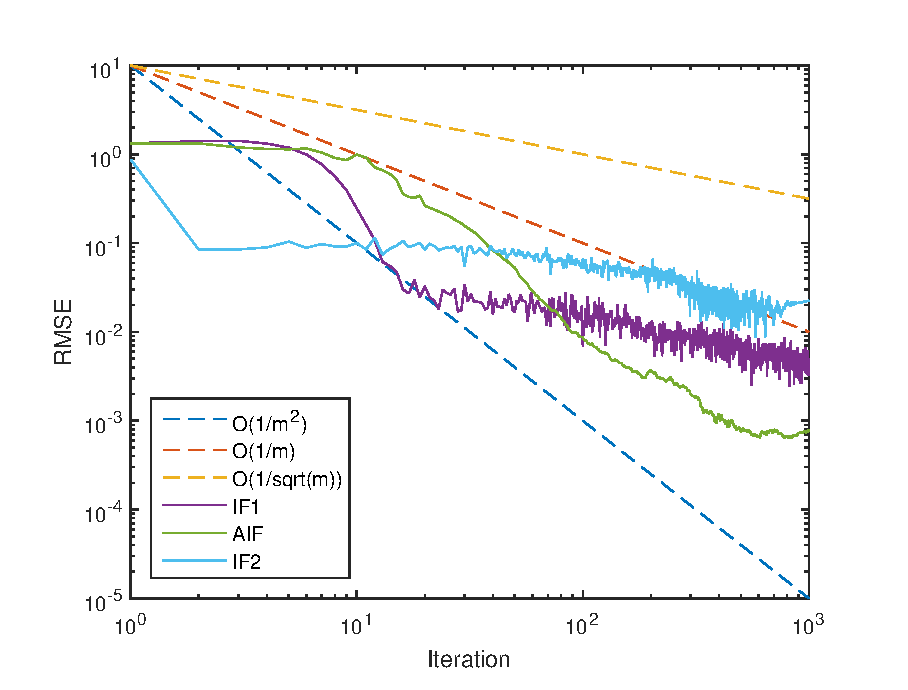
\includegraphics[width=1\textwidth]{./fig_simple_AR1/conv_plot}
  \caption{Shows the RMSE (i.e $\mid \hat{\theta}^{ML} - \hat{\theta}^{IF}\mid$ calculated over 10 runs) for different versions of the IF algorithm. The algorithm parameter settings for the IF1, AIF and IF2 algorithm are presented in Table \ref{tab:par_settings_AR1}}
  \label{fig:conv_plot_AR1}
\end{figure}


\begin{figure}[h]
  \centering
    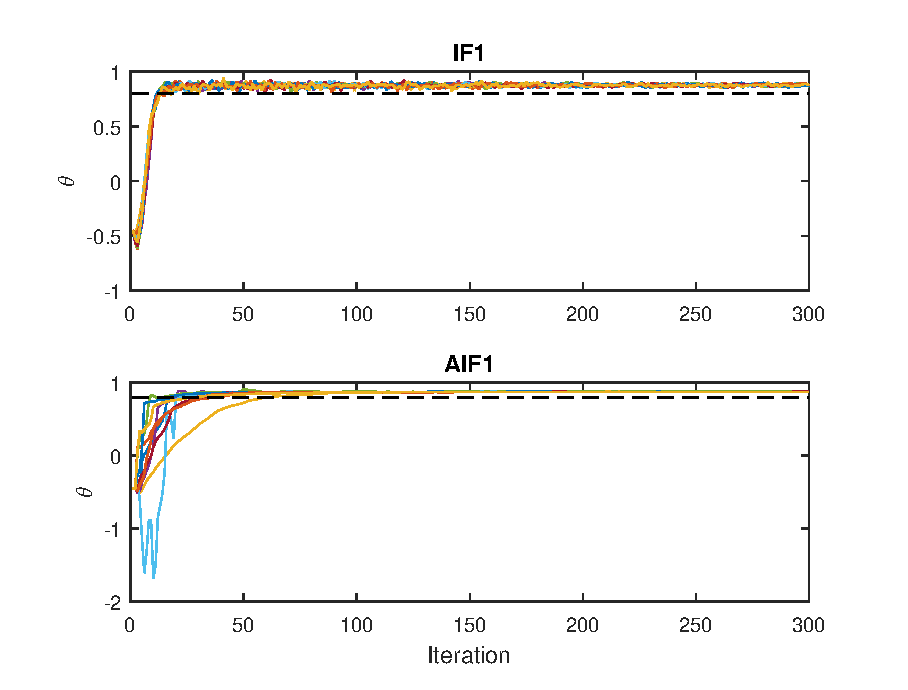
\includegraphics[width=1\textwidth]{./fig_simple_AR1/conv_theta_conv}
  \caption{Shows the convergence to the true value of the model parameter $\theta$ for different version of the IF algorithm  in the converging phase. The parameter settings for the IF1, IF2 and AIF algorithm are presented in Table \ref{tab:par_settings_AR1}}
  \label{fig:conv_theta_conv}
\end{figure}

\begin{figure}[h]
  \centering
    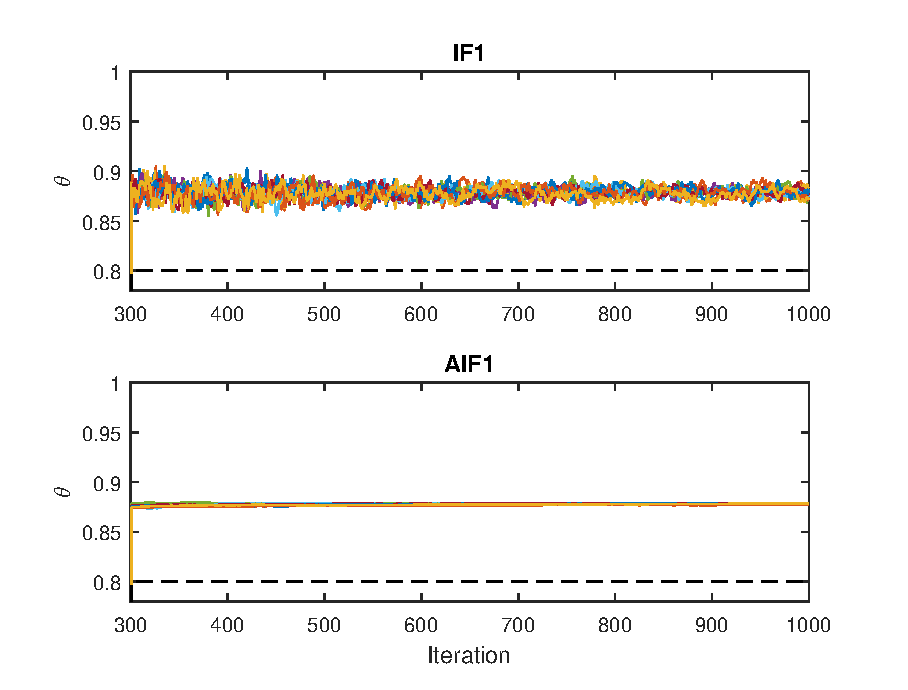
\includegraphics[width=1\textwidth]{./fig_simple_AR1/conv_theta_trans}
  \caption{Shows the convergence to the true value of the model parameter $\theta$ for different version of the IF algorithm in the transient phase. The algorithm parameter settings for the IF1, IF2 and AIF algorithm are presented in Table \ref{tab:par_settings_AR1}}
  \label{fig:conv_theta_trans}
\end{figure}


\begin{figure}[h]
  \centering
    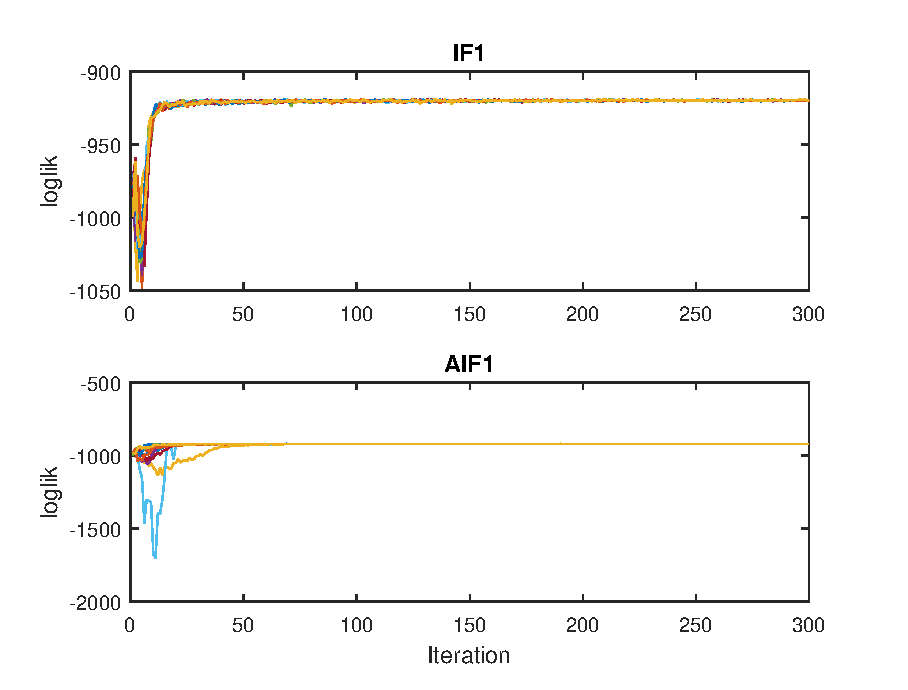
\includegraphics[width=1\textwidth]{./fig_simple_AR1/loglik_conv}
  \caption{Shows the log-likelihood values for different versions of the IF algorithm in the converging phase. The algorithm parameter settings for the IF1, AIF and IF2 algorithm are presented in Table \ref{tab:par_settings_AR1} }
  \label{fig:loglik_conv}
\end{figure}

\begin{figure}[h]
  \centering
    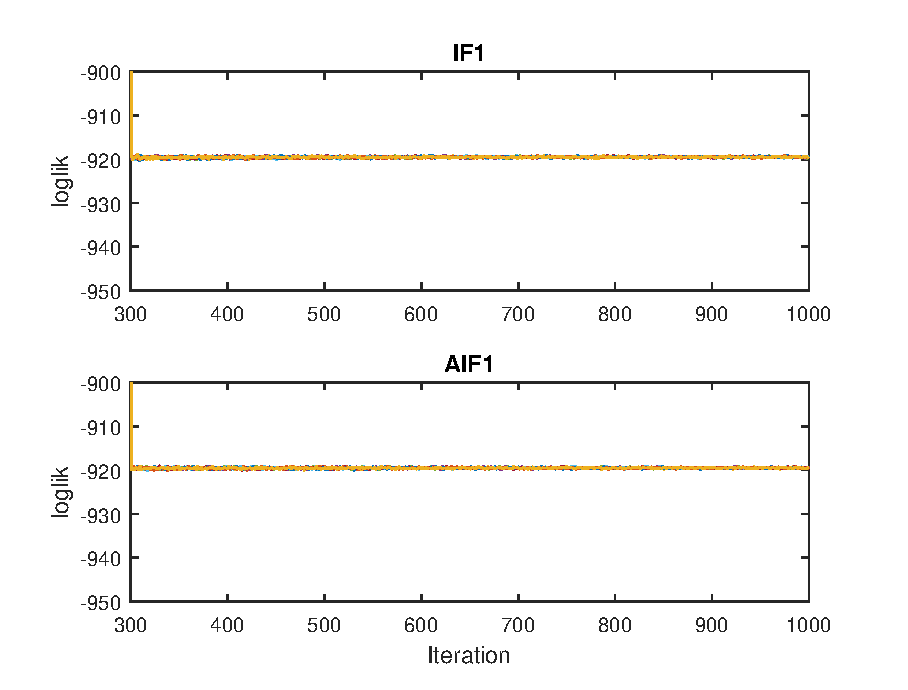
\includegraphics[width=1\textwidth]{./fig_simple_AR1/loglik_trans}
  \caption{Shows the log-likelihood values for different versions of the IF algorithm in the transient phase. The algorithm parameter settings for the IF1, IF2 and AIF algorithm are presented in Table \ref{tab:par_settings_AR1}}
  \label{fig:loglik_trans}
\end{figure}

\begin{figure}[h]
  \centering
    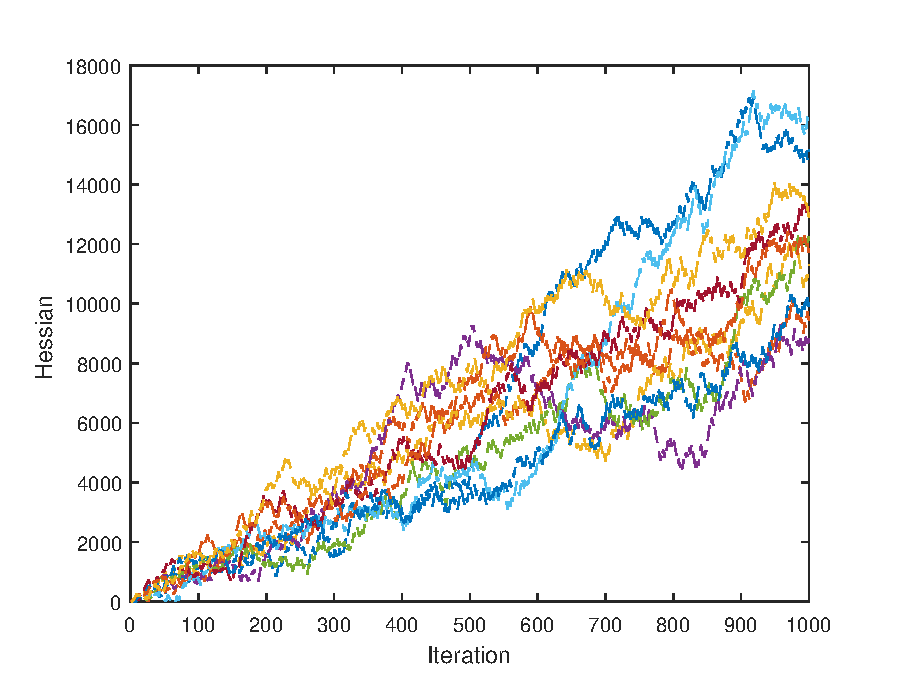
\includegraphics[width=1\textwidth]{./fig_simple_AR1/hessian_approx}
  \caption{Shows the approximation of the Hessian  for each iterations for 10 runs of the AIF algorithm. The algorithm parameter settings for the AIF algorithm are presented in Table \ref{tab:par_settings_AR1} }
  \label{fig:hessian_AR1}
\end{figure}


%%%%%%%%%%%%%%%%%%%%%%%%%%%%%%%%%%%%%%%%%%%%%%%%%%%%%%%%%%%%%%%%%%%%%%%%%%%%%%%%%%%%%%%%%%%%%%%%%%%%%%%%%
%%%%%                           GOMPERTZ MODEL                                                      %%%%%    
%%%%%%%%%%%%%%%%%%%%%%%%%%%%%%%%%%%%%%%%%%%%%%%%%%%%%%%%%%%%%%%%%%%%%%%%%%%%%%%%%%%%%%%%%%%%%%%%%%%%%%%%%
\section{The Gompertz Model}

The Gompertz model is a discrete time model for population growth \cite{ionides2015inference}. The Markov process $X_t$ in the Gompertz model is the population density and the observation process $Y_t$ is the population density, which is observed on an logarithmic scale and with an error. The model is presented in Equation \ref{eq:gompertz_model}

\begin{align} \label{eq:gompertz_model}
\begin{cases}
    X_{t + \Delta t} &= K^{1-e^{-r \Delta t}} X_{t}^{e^{-r \Delta t}} \epsilon_t \\
    \log Y_t &\sim \mathcal{N} ( \log X_t, \tau )
\end{cases}
\end{align}

In Equation \ref{eq:gompertz_model} are the $\epsilon_t$'s independently identically distributed random variable such that $\log \epsilon_t \sim \mathcal{N} (0, \sigma)$. The length of the time step $\Delta t$ is assumed to be $1$. If the Markov process $X_t$ is also transformed into the logarithmic scale the model then follows


\begin{align} \label{eq:gompertz_model_log}
\begin{cases}
    \log X_{t + \Delta t} &\sim \mathcal{N} ( (1-e^{-r \Delta t}) K + e^{-r \Delta t} X_{t}, \sigma) \\
    \log Y_t &\sim \mathcal{N} ( \log X_t, \tau )
\end{cases}
\end{align}


The transformed version of the Gompertez model in Equation \ref{eq:gompertz_model_log} is convenient since it allows exact maximum likelihood estimation of the model parameters by employing a Kalman filter  \cite{ionides2015inference}. However, in this thesis is the Gompertz model  only considered in the non-transformed version in Equation \ref{eq:gompertz_model}. 

The model parameters $r$, $\sigma$ and $\tau$ are estimated using the IF1, IF2 and AIF algorithm, but the parameter $K$ is assumed to be known. However, since the model parameters have to be strictly large then zero the model parameters are transformed with the logarithm function to facilitate the estimation of the model parameters and transfer the allowed range of the parameter from $[ 0 \,\, \infty]$ to the whole real axis.   

For the Gompertz mode is the mapping in Equation \ref{eq:mapping2} used to ensure a semi-positive Hessian matrix. The mapping in Equation \ref{eq:mapping2} is used to avoid problems with obtaing a complex matrix after calculating the square root in Equation \ref{eq:mapping1}


\subsection{Simulation Results for the Gompertz Model}

For the Gompertz model is the \textit{simulators} $f_{X_0}$ and $f_{X_n \mid X_{n-1}}$, and the \textit{evaluator} $f_{Y_n \mid X_n}$ set to 

\begin{align} \label{eq:simple_AR_model}
\begin{cases}
    f_{X_0} &= \mathcal{U}(0,1) \\
    f_{X_n \mid X_{n-1}} &= K^{1-e^{-r \Delta t}} X_{t}^{e^{ -r \Delta t }} \epsilon_t, \, \text{where} \, \log \epsilon_t \sim \mathcal{N} (0, \sigma) \\
    f_{Y_n \mid X_n} &= f(y^{*}_{n} \mid \log X_t , \tau) \footnotemark 
\end{cases}
\end{align}

\footnotetext{$f(y^{*}_n \mid \log X_t , \tau)$ is the normal probability density function $f(x \mid \mu, \sigma)$ }

The algorithm parameters for the IF1, IF2 and AIF algorithm are presented in Table \ref{tab:par_settings_Gompertz}. The \textit{start values} are drawn form a uniform distribution on $[0 \, 1]$. The model parameter estimations are computed on the same data as in \cite{king2015statistical}. This is done to be able to compare the estimated model parameters with the exact maximum likelihood estimation of the model parameters that are provided in  \cite{king2015statistical}. 

% Skriva något om burn in period!!!

\begin{table}[h]
    \centering
    \caption{Presents the model parameter settings for the IF1, AIF and IF2 algorithm for the Gompertz model }
    \resizebox{\columnwidth}{!}{% % scale to fit page!

    \begin{tabular}{ c  c | c  c | c  c }
    \toprule
        \multicolumn{2}{c}{IF1} & \multicolumn{2}{c}{AIF} & \multicolumn{2}{c}{IF2} \\ 
    \midrule
        Parameter   &   Value              & Parameter     & Value                    & Parameter & Value \\
        $M$         &   1000               &     $M$       & 200  + 5                   & $M$       &   1000    \\   
        $N$         &   100                &     $N$       &  100                     & $N$       & 100 \\
        $\delta$       &   1       &      $\delta$    &  2            & $J$       & 1000   \\
        $J_m$    &   $50 \cdot m$     &   $\J_m$    &  $50 \cdot m$         & $\sigma_m$  &  $0.001 \cdot 0.99^{m-1}$   \\
        $\tau_m$    &   $\sqrt{m^{-1}}$                   & $\tau_m$       & $\sqrt{m^{-1}}$                        &             &   \\    
        $\sigma_m$    &   $\sqrt{m^{-0.5-\delta}}$                  & $\sigma_m$    & $\sqrt{m^{-0.5-\delta}}$ &             &       \\
        $\alpha$         &   1                &$a_m$       &    $\frac{50}{(1+m+0.05 \cdot M)^{0.9}}$                    &             &    \\
        $a$         &   0.02     &  $c_m$       & $\frac{std(y^{*}) \cdot 2}{(m+1)^{0.2}}$  &           &       \\
        $A$       &   $0.05 \cdot M$  &  $\Delta_m$  & Bernoulli $\pm 1$   &           &                 \\ 
        $a_m$  &   $\frac{a}{(1+m+A)^{0.9}} $    &  $\delta_m$    &    $10000 \cdot m$                        &           &       \\
        $\Sigma$    &   $\scalemath{0.8}{\begin{pmatrix} 
       0.02 & 0 & 0 \\
       0 & 0.02 & 0 \\
       0 & 0 & 0.02
     \end{pmatrix}}$               &       $\Sigma$          &          $\scalemath{0.8}{\begin{pmatrix} 
       0.02 & 0 & 0 \\
       0 & 0.02 & 0 \\
       0 & 0 & 0.02
     \end{pmatrix}}$                  &           &       \\ 
        \bottomrule
    \end{tabular}
    }
    \label{tab:par_settings_Gompertz}
\end{table}



\subsubsection{Estimating three parameters}

The model parameters $r$, $\sigma$ and $\tau$ are first estimated using the IF1, IF2 and AIF algorithm. The obtained model parameter estimations, as well as the maximum likelihood estimation of the parameters are presented in Table \ref{tab:par_Gompertz}. From Table \ref{tab:par_Gompertz} is it possible to conclude that it is only the IF1 and IF2 algorithm that generates reasonable model parameter estimations when three model parameters are estimated. The estimation of the parameter $r$ also seems to be better for the IF1 and IF2 model compared to the maximum likelihood estimation since the true value for all model parameters is $0.1$. 

The convergence of the IF1, IF2 and AIF algorithm is presented in Figure \ref{fig:cov_three_par}, where the model parameter estimation for each iteration is shown. It is clear that only the IF1 and IF2 algorithms converge. The model parameter estimation of the AIF algorithm does converge, but it does not converge to the correct value. It is also notable the the model parameter estimation of the AIF algorithm only moves very little away from the start value.     

\begin{table}[h]
    \centering
    \caption{Presents the obtained model parameter estimation for the IF1, IF2 and AIF algorithm where three model parameters in the Gompertz model are estimated. The model parameter estimations are calculated as the mean of the parameter estimations over 10 runs of the algorithms.  Also presented the exact  maximum likelihood estimation of the model parameters for the Gompertz model \cite{king2015statistical}  }
    \begin{tabular}{ c | c c  c }
    \toprule
        & $r$ & $\sigma$ & $\tau$ \\ 
    \midrule
    IF1  & 0.1663  &  0.1675 &    0.1607 \\ 
    IF2  & 0.1458  &  0.1534 &    0.1500 \\ 
    AIF  & 0.6280  &  0.6656 &    0.6108 \\
    Exact ml  \cite{king2015statistical} & 0.0322 & 0.0694 & 0.1170 \\ 
    \bottomrule
    \end{tabular}
    \label{tab:par_Gompertz}
\end{table}



\begin{figure*}
        \centering
        \begin{subfigure}[b]{0.7\textwidth}
            \centering
            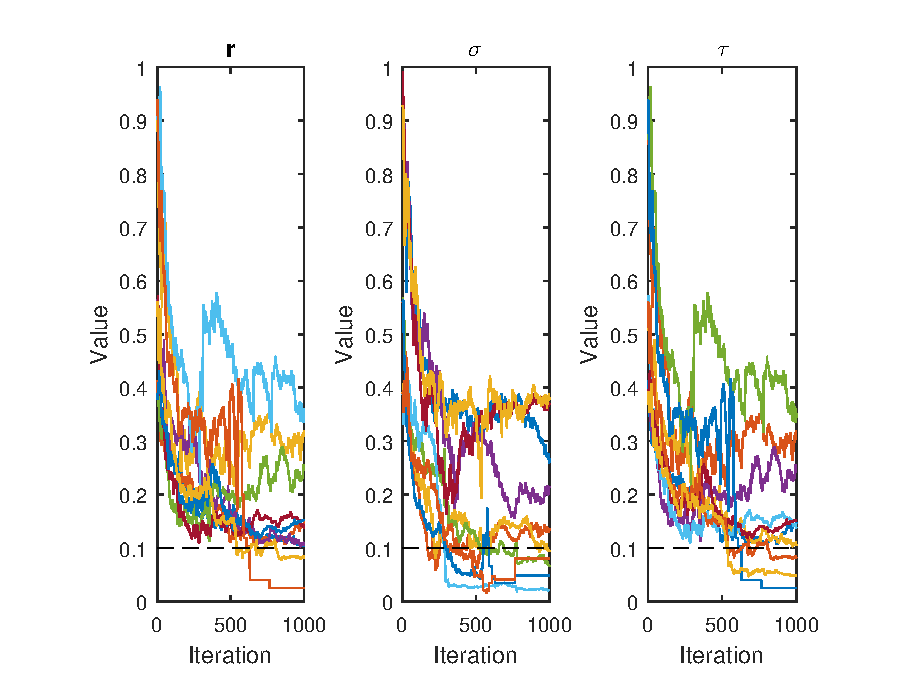
\includegraphics[width=\textwidth]{./fig_gompertz/IF1_3_par}
            \caption[]%
            { \small IF1 }     
            \label{fig:mean and std of net14}
        \end{subfigure}
        %\hfill
        \begin{subfigure}[b]{0.7\textwidth}  
            \centering 
            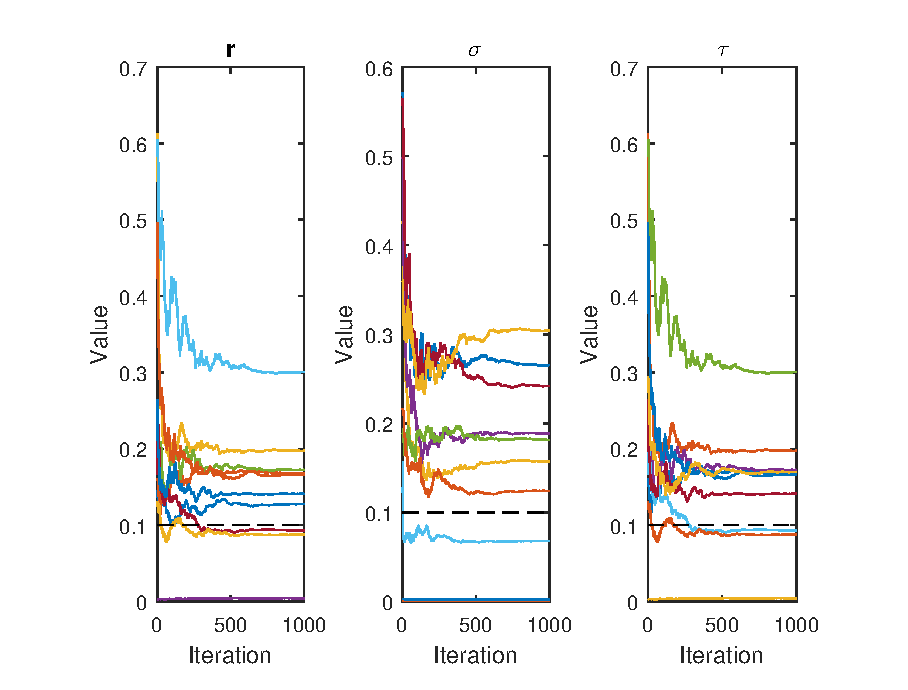
\includegraphics[width=\textwidth]{./fig_gompertz/IF2_3_par}
            \caption[]%
            { \small IF2 }     
            \label{fig:mean and std of net24}
        \end{subfigure}
        %\vskip\baselineskip
        \begin{subfigure}[b]{0.7\textwidth}   
            \centering 
            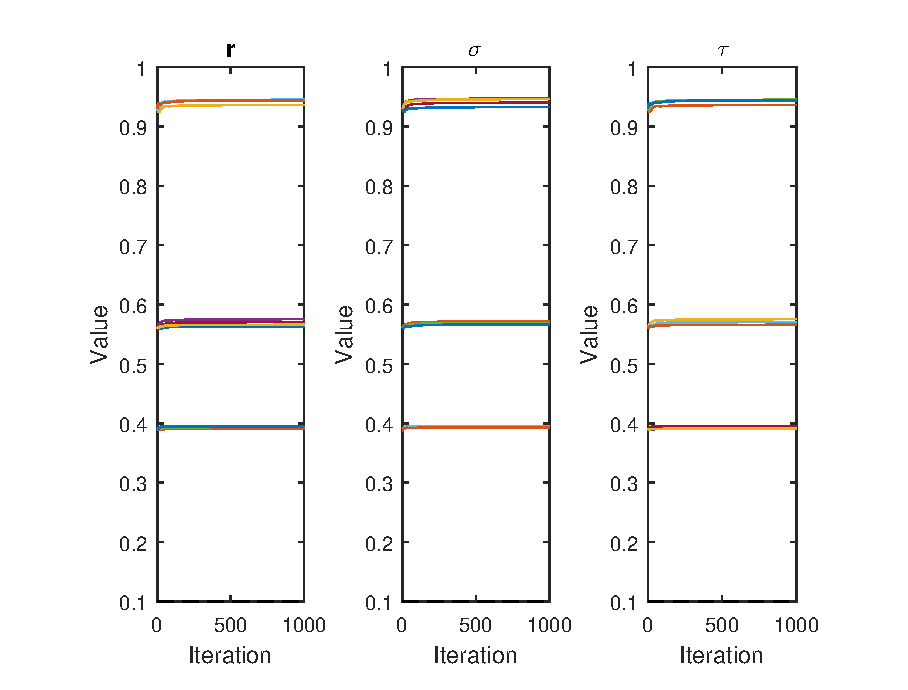
\includegraphics[width=\textwidth]{./fig_gompertz/AIF_3_par}
            \caption[]%
            { \small AIF } 
            \label{fig:mean and std of net34}
        \end{subfigure}
        \caption[ ]
        {\small Convergence for the IF1, IF2 and AIF algorithm where three model parameters in the Gompertz model are estimated. The algorithm parameter settings  are presented in Table \ref{tab:par_settings_Gompertz} }
        \label{fig:cov_three_par}
\end{figure*}

\subsubsection{Estimating two parameters}

The estimation results obtained when estimating three model parameters were not satisfying. The next step is therefore to only estimate the parameters $\sigma$ and $\tau$ and treat the model parameter $r$ as known. The obtained model parameter estimations, as well as the exact maximum likelihood estimation of the parameters are presented in Table \ref{tab:par2_Gompertz}. From Table \ref{tab:par2_Gompertz} is it  possible to conclude that only the IF1 and IF2 algorithms  generate reasonable model parameter estimations when two model parameters are estimated. 

The convergence of the IF1, IF2 and AIF algorithm is presented in Figure \ref{fig:cov_two_par}, where the model parameter estimation for each iteration is shown. The IF1 algorithm  seems to converge quite nicely to the true model parameter. The IF2 algorithm also seems to converge quite well. However, both the IF1 and IF2 algorithm seem to  better estimate the model parameter $\tau$, then the model parameter $\sigma$. Hence, the IF1 and IF2 algorithms only generate good model parameter estimations for one of the two model parameters.
The AIF algorithm on the other hand does not converge to true model parameters. The AIF algorithm instead seems to converge to some other model parameter value. Hence, the performance of the algorithms are only slightly improved when only two parameters are estimated and AIF algoirthms still does not generate reliable model parameter estimations.   

\begin{table}[h]
    \centering
    \caption{Presents the obtained model parameter estimation for the IF1, IF2 and AIF algorithm where two model parameters in the Gompertz model are estimated. The model parameter estimations are calculated as the mean of the parameter estimations over 10 runs of the algorithms.  Also presented the exact  maximum likelihood estimation of the model parameters for the Gompertz model \cite{king2015statistical} }
    \begin{tabular}{ c | c c }
    \toprule
        & $\sigma$ & $\tau$ \\ 
    \midrule
    IF1  & 0.2634 &   0.1359\\ 
    IF2  & 0.2039 &   0.1136 \\ 
    AIF  & 0.2663 &   0.9507 \\
    Exact ml \cite{king2015statistical}  & 0.0694 & 0.1170 \\ 
    \bottomrule
    \end{tabular}
    \label{tab:par2_Gompertz}
\end{table}


\begin{figure*}
        \centering
        \begin{subfigure}[b]{0.7\textwidth}
            \centering
            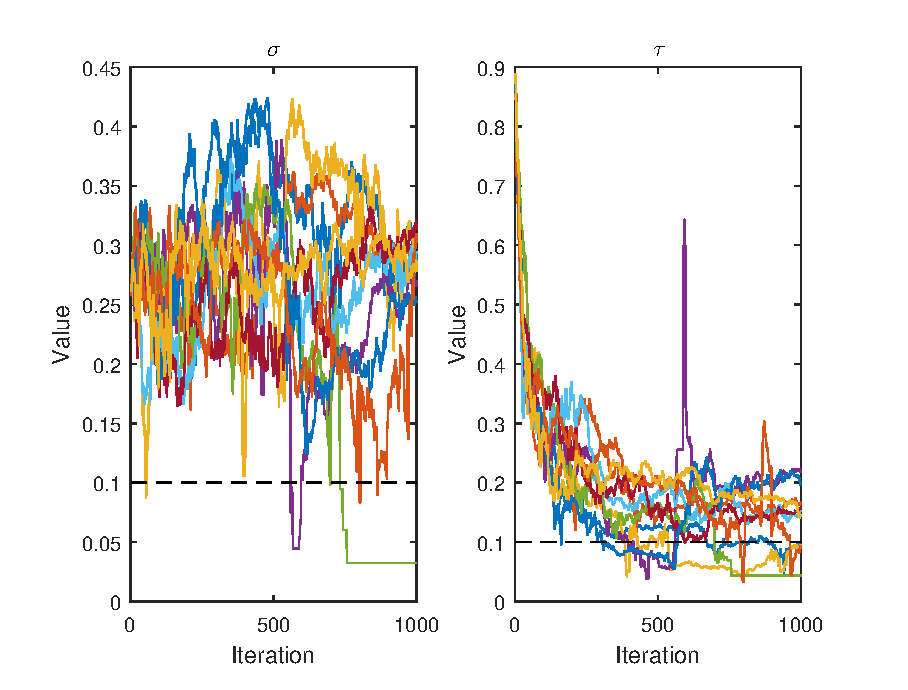
\includegraphics[width=\textwidth]{./fig_gompertz/IF1_2_par}
            \caption[]%
            { \small IF1 }     
            \label{fig:mean and std of net14}
        \end{subfigure}
        %\hfill
        \begin{subfigure}[b]{0.7\textwidth}  
            \centering 
            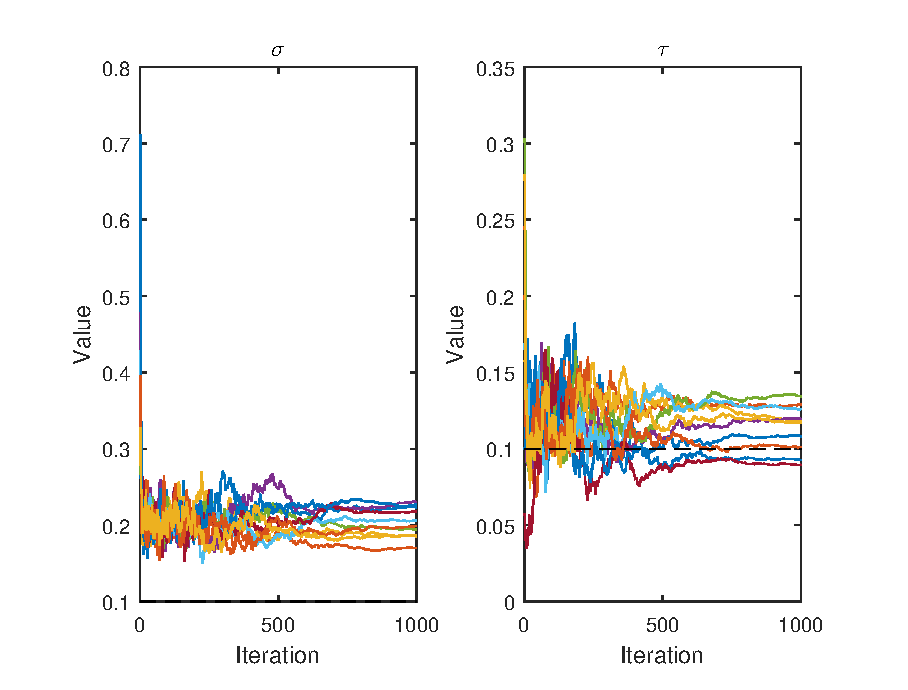
\includegraphics[width=\textwidth]{./fig_gompertz/IF2_2_par}
            \caption[]%
            { \small IF2 }     
            \label{fig:mean and std of net24}
        \end{subfigure}
        %\vskip\baselineskip
        \begin{subfigure}[b]{0.7\textwidth}   
            \centering 
            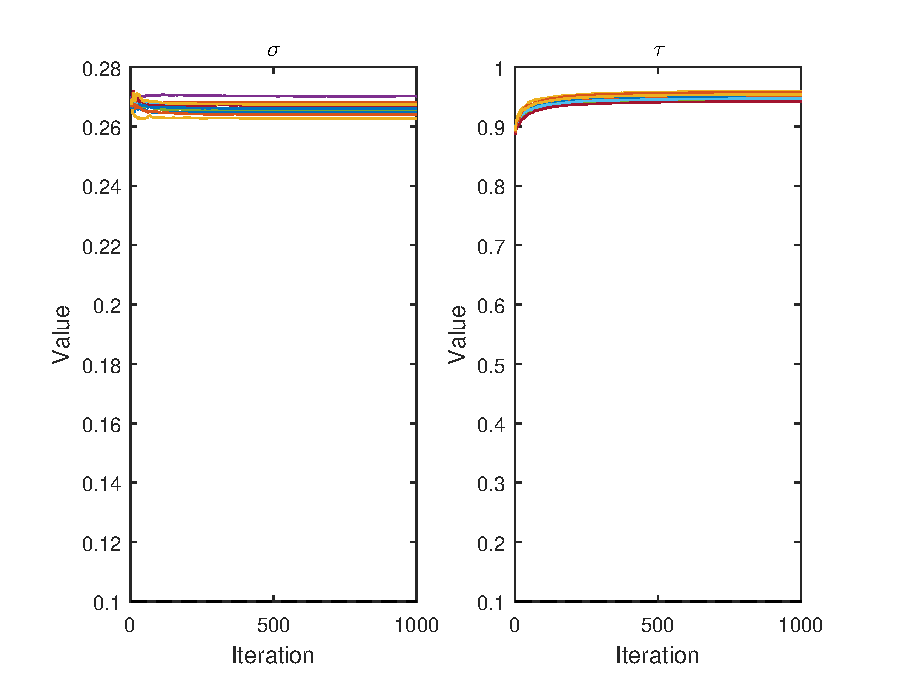
\includegraphics[width=\textwidth]{./fig_gompertz/AIF_2_par}
            \caption[]%
            { \small AIF } 
            \label{fig:mean and std of net34}
        \end{subfigure}
        \caption[ ]
        {\small Convergence for the IF1. IF2 and AIF algorithm where two model parameters in the Gompertz model are estimated. The algorithm parameter settings are presented in Table \ref{tab:par_settings_Gompertz} }
        \label{fig:cov_two_par}
\end{figure*}

\subsubsection{Conclusion regarding the Gompertz model}
The conclusion is that both the IF1 and IF2 algorithms generate reasonable model parameter estimations for the Gompertz model. However, the AIF algorithm does not generate reliable model parameter estiamtions since the AIF algorithm  does not converge to the true model parameters, this is likeliy due to the poor estiamtion of the Hessian matrix in the AIF algorithm. 


%%%%%%%%%%%%%%%%%%%%%%%%%%%%%%%%%%%%%%%%%%%%%%%%%%%%%%%%%%%%%%%%%%%%%%%%%%%%%%%%%%%%%%%%%%%%%%%%%%%%%%%%%
%%%%%                           The SIR Model                                                      %%%%%    
%%%%%%%%%%%%%%%%%%%%%%%%%%%%%%%%%%%%%%%%%%%%%%%%%%%%%%%%%%%%%%%%%%%%%%%%%%%%%%%%%%%%%%%%%%%%%%%%%%%%%%%%%



\section{The SIR Model}

% introduction to SIR
The SIR model is an  epidemiological model used to model how a disease spreads in a population of hosts. The model consists of four classes, \textit{number susceptible} ($S$), \textit{number infectious} ($I$) and \textit{number recovered} (immune) ($R$) . A diagram for the SIR model is presented at Figure \ref{fig:diagram_SIR_model}. \cite{king2015statistical}  

\begin{figure}[ht]
  \centering
    \includegraphics[width=1\textwidth]{./fig_sir/fig_SIR_model}
  \caption{The diagram show the SIR model. Where $S$ is \textit{number susceptible}, $I$ \textit{number infectious} and $R$ \textit{number recovered} (immune) and total population $N = S + I + R$. The parameter $\mu$ is the birth/death   rate, $\lambda (t) = \beta \frac{I(t)}{P}$ is the force of infection, $\gamma$ is the recovery rate. The parameter $\rho$ is the probability of which new infections are recorded. Source \cite{king2015statistical}}
  \label{fig:diagram_SIR_model}
\end{figure}

The SIR model can be viewed as a POMP model where the Markov process $X_t$ consists of the processes $S$, $I$ and $R$, while the observation process $Y_t$ is the process $C$. The dynamic for the Markov process $X_t$ (i.e for the processes S, I and R) is

\begin{align} \label{eq:SIR_model_X}
\begin{cases}
    \frac{dS}{ dt } = \mu (N - S) - \beta \frac{I}{N} S \\
    \frac{dI}{dt} = \beta \frac{I}{N} S - \gamma I - \mu I \\
    \frac{dR}{dt} = \gamma I - \mu R
\end{cases}
\end{align}

The number of cases on a time interval $[ t_1 , t_2 ]$ is assumed to be negative binomial distributed

\begin{align} \label{eq:SIR_model_Y}
    C(t_1 , t_2 ) \sim negbin( \rho \Delta_{I \rightarrow  R} (t_1 , t_2 ), \theta )
\end{align}

In Equation \ref{eq:SIR_model_Y} is $\rho \Delta_{I \rightarrow  R} (t_1 , t_2 )$  the mean for the negative binomial distribution and $\theta$ is the shape parameter.

The SIR model is fully described by the model parameters, $\mu$, $\beta$, $\gamma$, $\rho$ and $\theta$. However, $\mu$ governs the birth/death rate and is therefore not linked to the specifications of the disease. Furthermore, the model parameter $\theta$ is the shape parameter for the negative binomial distribution and therefore does not  have a direct affect on the dynamic of the disease.  The parameters  $\beta$, $\gamma$ and $\rho$ are however directly linked to the specifications of the disease. The objective in this thesis is therefore  to estimate the parameters $\beta$, $\gamma$ and $\rho$. The model parameter $\rho$ can only take values on the interval $[ 0 \,\, 1]$ and the model parameter $\rho$ is therefore transformed by the  cumulative distribution function of the standard normal distribution to facilitate the estimation of the $\rho$ parameter, which transfers the allowed range of the parameter $\rho$ from $[ 0 \,\, 1]$ to the whole real axis.   

\subsection{Simulation Results for the SIR Model}

The \textit{simulator} $f_{X_0}$,  and \textit{evaluator} $f_{Y_n \mid X_n}$ for the SIR model are 

\begin{align} \label{eq:simple_AR_model}
\begin{cases}
    f_{X_0} &= \mathcal{N} \Big( $\scalemath{0.6}{\begin{pmatrix} 
       30000 & 0 & 0 & 0 \\
       0 & 800 & 0 & 0 \\
       0 & 0 & 470000 & 0 \\
       0 & 0 & 0 & 400
     \end{pmatrix}}$,$\scalemath{0.6}{\begin{pmatrix} 
       50 & 0 & 0 & 0 \\
       0 & 30 & 0 & 0 \\
       0 & 0 & 500 & 0 \\
       0 & 0 & 0 & 10
     \end{pmatrix}}$ \Big) \\
    f_{Y_n \mid X_n} &= f( y^{*}_n \mid \rho H, \theta ) \footnotemark \,\, \text{where} \,\, H = \Delta_{I \rightarrow  R}  
\end{cases}
\end{align}

\footnotetext{$f( y^{*}_n \mid \rho H, \theta  )$ is the negative binomial  distribution function $f(x \mid \mu, \theta)$} %where $\mu$ is the mean and $\theta$ the shape parameter }

The  \textit{simulator} $f_{X_n \mid X_{n-1}}$ for the SIR model follows a Euler-multinational distribution. The process $X_n$ is advanced one time step by employing the Euler-method and by simulating the system in Equation \ref{eq:SIR_model_X} over one time step. A more detailed outline of the Euler-multinational distribution and the Euler-method can be found in \cite{king2015statistical}.  

Before estimating the model parameters is the  data $y^{*}$   generated by simulating the system in described in Equation \ref{eq:SIR_model_X} and Figure \ref{fig:diagram_SIR_model}. The simulated $X_t$ process is presented in Figure \ref{fig:sim_X_sir} and the data $y^{*}$ (i.e. the process for the number of cases) is presented in Figure \ref{fig:sim_Y_sir}

The algorithm parameter settings used for the IF1, IF2 and AIF algorithm are presented in Table \ref{tab:par_settings_sir}.

For the SIR mode is the mapping in Equation \ref{eq:mapping2} used to ensure a semi-positive Hessian matrix. The mapping in Equation  \ref{eq:mapping2} is used to avoid problems with obtaining a complex matrix after calculating the square root in Equation \ref{eq:mapping1}


\begin{table}[h]
    \centering
    \caption{Presents the algorithm parameter settings for the IF1, AIF and IF2 algorithm for the SIR model }
    \resizebox{\columnwidth}{!}{% % scale to fit page!
    \begin{tabular}{ c  c | c  c | c  c }
    \toprule
    \multicolumn{2}{c}{IF1} & \multicolumn{2}{c}{AIF} & \multicolumn{2}{c}{IF2} \\ 
    \midrule
        Parameter   &   Value              & Parameter     & Value                    & Parameter & Value \\
        $M$         &   50               &     $M$       & 200  + 1                   & $M$       &   50    \\   
        $N$         &   500                &     $N$       &  100                     & $N$       & 500 \\
        $\delta$       &   2       &      $\delta$    &  2            & $J$       & 1000   \\
        $\J_m$    &   $50 \cdot m$     &   $\J_m$    &  $50 \cdot m$         & $\sigma_m$  &  $1 \cdot 0.99^{m-1}$   \\
        $\tau_m$    &   $\sqrt{m^{-1}}$                   & $\tau_m$      & $\sqrt{m^{-1}}$                        &             &   \\    
        $\sigma_m$    &   $\sqrt{m^{-0.5-\delta}}$                   & $\sigma_m$    & $\sqrt{m^{-0.5-\delta}}$ &             &       \\
        $\alpha$         &  1               &$a_m$       & $\frac{\begin{pmatrix} 
       10 & 5 & 0.5 \\\end{pmatrix}}{(m + 0.05 \cdot M)^{0.9}}$                     &             &    \\
        $a$         &   $\begin{pmatrix} 
       20 & 1 & 0.01 \\
     \end{pmatrix}$       &  $c_m$        & $\frac{std(y^{*}) \cdot 2}{(m+1)^{0.2}}$           &       \\
        $A$       &   $0.05 \cdot M$  &  $\Delta_m$  & Bernoulli $\pm 1$   &           &                 \\ 
        $A_m$  &    $\frac{a}{(1+m+A)^{\alpha}}$      &  $\delta$    &    $10000 \cdot m$                        &           &       \\
        $\Sigma$    &  $\scalemath{0.8}{\begin{pmatrix} 
       20 & 0 & 0 \\
       0 & 0.2 & 0 \\
       0 & 0 & 0.2
     \end{pmatrix}}$               &      $\Sigma$           &        $\scalemath{0.8}{\begin{pmatrix} 
       20 & 0 & 0 \\
       0 & 0.2 & 0 \\
       0 & 0 & 0.2
     \end{pmatrix}}$                     &           &       \\ 
    \bottomrule
    \end{tabular}
    }
    \label{tab:par_settings_sir}
\end{table}



\begin{figure}[ht]
  \centering
    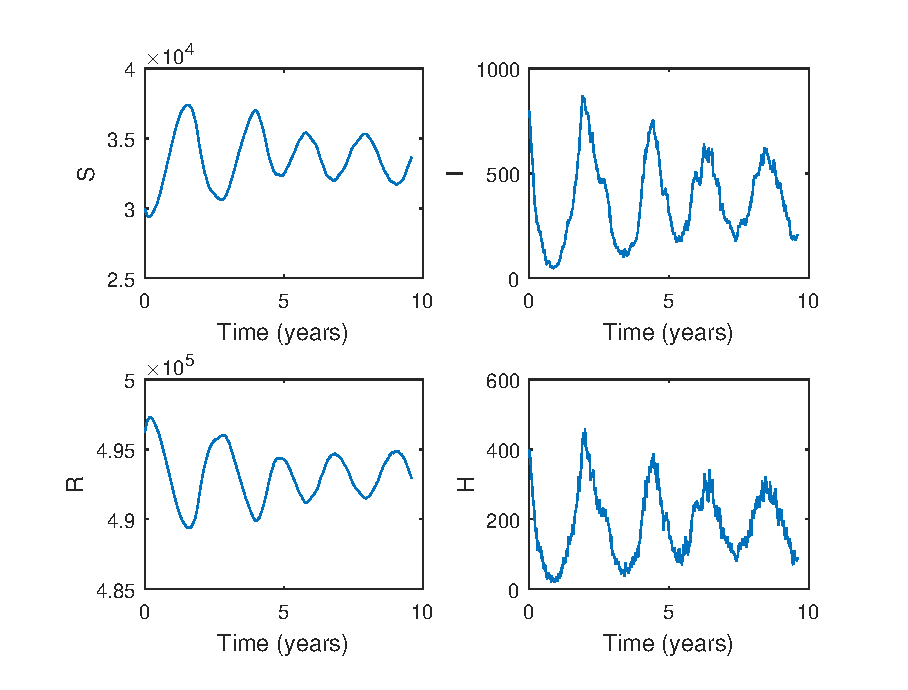
\includegraphics[width=1\textwidth]{./fig_sir/X_sim}
  \caption{Simulated $X_t$ process for the SIR model}
  \label{fig:sim_X_sir}
\end{figure} 

\begin{figure}[ht]
  \centering
    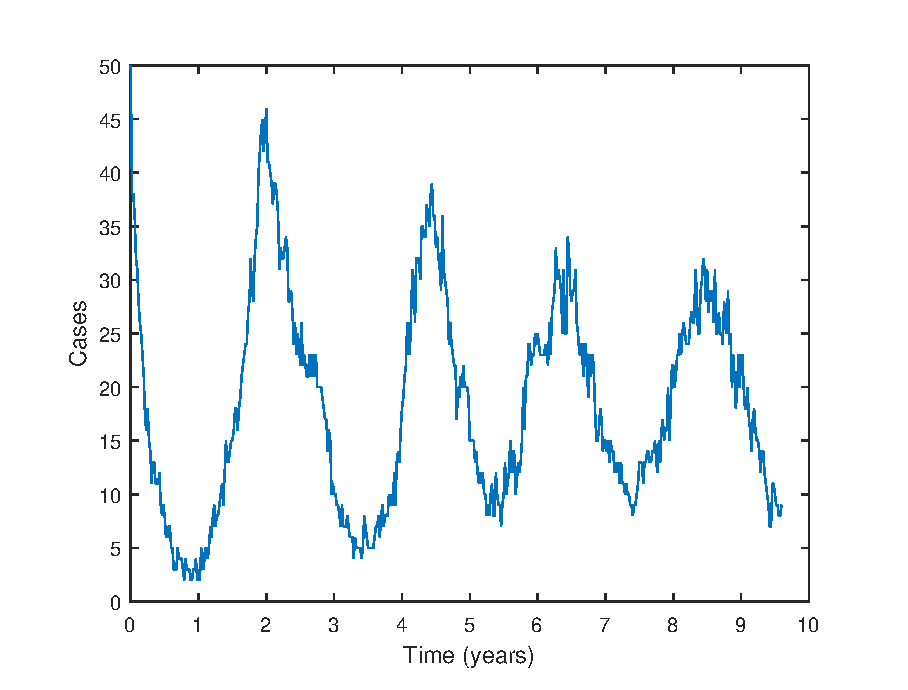
\includegraphics[width=1\textwidth]{./fig_sir/Y_sim}
  \caption{Simulated data $y^{*}$ (i.e. number of cases $C$) for the SIR model}
  \label{fig:sim_Y_sir}
\end{figure} 

The simulation results are presented in Figure \ref{fig:res_IF1}, \ref{fig:res_IF2} and \ref{fig:res_AIF}. In Figure \ref{fig:res_IF1} and \ref{fig:res_IF2} it is notable that both the IF1 and the IF2 algorithm can estimate the $\rho$ parameter quite well. For the IF1 algorithm is the estiamtion of the $\gamma$ parameter also quite good. However non of the models manage to estimate the $\beta$ parameter with any high precision. While the IF1 and IF2 algorithms seem to converge the parameter estiamtions of the AIF algorithm generally do not seem to converge. Only the estiamtion of the $\gamma$ parameter for the AIF model seem to converge while the estiamtion of the $\beta$ and $\rho$ parameter do not converge.  

\begin{figure}[h]
  \centering
    \includegraphics[width=1\textwidth]{./fig_sir/IF1}
  \caption{Shows the convergence of the model parameters $\beta$, $\gamma$ and $\rho$ for the SIR model using the IF1 algorithm computed over 10 runs of the algorithm. The algorithm parameter settings for the IF1 algorithm are presented in Table \ref{tab:par_settings_sir} }
  \label{fig:res_IF1}
\end{figure}

\begin{figure}[h]
  \centering
    \includegraphics[width=1\textwidth]{./fig_sir/IF2}
  \caption{Shows the convergence of the model parameters $\beta$, $\gamma$ and $\rho$ for the SIR model using the IF2 algorithm computed over 10 runs of the algorithm. The algorithm parameter settings for the IF2 algorithm are presented in Table \ref{tab:par_settings_AR1} }
  \label{fig:res_IF2}
\end{figure}

\begin{figure}[h]
  \centering
    \includegraphics[width=1\textwidth]{./fig_sir/AIF}
  \caption{Shows the convergence of the model parameters $\beta$, $\gamma$ and $\rho$ for the SIR model using the AIF algorithm computed over 10 runs of the algorithm. The algorithm parameter settings for the AIF algorithm are presented in Table \ref{tab:par_settings_AR1} }
  \label{fig:res_AIF}
\end{figure}


\section{Summary of Simulation Results}
% summerare ihop resulatet på en sida ish 
The three different models used for simulations are quite different. The simple AR(1) model is a model driven by the noise terms and the SIR model is a dynamical model, while the Gompertz model is model with both dynamical and noise driven parts. The complexity of the models also varies where the Simple AR(1) model is the least complex model and the SIR model the most complex mode. The three models  were  chosen because of their different characteristics. 

The conclusions from the simulation studies  are.   

\newcounter{para}
\newcommand\mypara{\par(\refstepcounter{para}\thepara)\space}


\mypara \textit{ AIF is only efficient for the Simple AR(1) model } From the simulation results is it clear that the AIF algorithm is only comparable with the IF1 algorithm for the simple AR(1) model.  The performance of the AIF algorithm is also considerable worse compared to the IF1 algorithm for the other models.
% Länka till figurer och förklara varför



\mypara \textit{ The Hessian approximation is poor } The poor performance of the AIF model is probably due to the fact that the approximation of the Hessian matrix is quite bad. This obersvation is possible to draw since [hur den approximativet hessianen relaterar till den verkliga hessianen]. A problematic part with approximation of the Hessian matrix is the mapping in Equation \ref{eq:mapping2} that is used for the Gompertz and SIR model. To ensure a semi-definite matrix with using this mapping the $\delta_m$ has to be very large to counteract the non-positive elements of the matrix $\overbar{H}_m$. Hence, the matrix $\overbar{H}_m$ undergoes a quite large transformation to ensure a semi-definite matrix and it is therefore possible that important information in the matrix $\overbar{H}_m$ is partly lost. 



\mypara \textit{ The IF1 algorithm seems to generate the best model parameters estimations } An interesting finding is that the IF1 algorithm seems to be the algorithm that generates the best model parameter estimations. However, the objective of this thesis is not to compare the IF1 and IF2 algorithm so this finding is not further analysed but rather noticed. 

% Länka till figurer och ta visa på dettan 

\chapter{Discussion} \label{chap:discussion}

This chapter contains a general discussion on the Iterated Filtering algorithm and also a specific discussion on the Adaptive Iterated Filtering algorithm. The chapter also discusses further research questions regarding the IF algorithm.   

\section{General Discussion on the Iterated Filtering Algorithm} \label{sec:disc_IF}
% borde hete disucssion

The Iterated Filtering algorithm is a suitable algorithm to compute maximum likelihood based parameter estimations of POMP models. However, the IF algorithm (both the IF1 and IF2 version of the Iterated Filtering algorithm), has two  main drawbacks. 

%\newcounter{para}
%\newcommand\mypara{\par(\refstepcounter{para}\thepara)\space}

\setcounter{para}{0} % reset para counter to 0 

\mypara \textit{Sensitive of choice of algorithm parameters} The IF algorithm is highly sensitive to algorithm parameter changes. Especially a well stated gain sequence is crucial to obtain an algorithm that is stable and that converges properly. Furthermore, even though guidelines are available is it not quite clear how the algorithm parameters for the IF1 and IF2 algorithms should be chosen to obtain a stable and optimal IF algorithm. This problem especially applies to the IF2 algorithm. 

\mypara \textit{Tuning} Since the IF algorithm is sensitive to algorithm parameter changes the algorithm requires quite a bit of tuning before a stable algorithm that converges properly is obtained. 

Hence, the IF algorithm is not an algorithm that can be applied to a problem straight away, but requires tuning and proper choices of algorithm parameters. 

The algorithm parameters for the IF1 algorithm are all easily interpreted and it is clear how they effect the algorithm. However, the connection between the algorithm parameters of the IF1 algorithm and the IF2 algorithm is not clear. Specifically the connection between the two perturbation sequences of the IF1 algorithm $\sigma_m$ and $\tau_m$ and the perturbation sequence $\sigma_m$ and perturbation density $h_m$ is unclear. Due to this reason and the fact that the IF1 and IF2 algorithm are two quite different versions of the Iterated Filtering algorithm are comparisons between the two algorithms hard to do and interpret. 

The main advantage of the IF algorithm is that the algorithm can be applied to a large amount of models in many different fields. It is also simple to implement the IF algorithm to a new model if the IF algorithm has been implemented once since the main different for the IF algorithm of different models are the specification of the simulators $f_{X_0}$ and $f_{X_{n+1} \mid X_n}$, and the evaluator $f_{Y_n \mid X_n}$. There also exists a R package that allows the user to apply the IF algorithm to a model of choice  with only specifying the model and not actually implementing the IF algorithm \cite{king2015statistical}. 

\section{Discussion on the Adaptive Iterated Filtering Algorithm}

The main idea of the Adaptive Iterated Filtering algorithm is to construct an IF algorithm with an optimal gain sequence. This is done by incorporating second-order information by approximating the Hessian matrix. 

The simulation results in Chapter \ref{chap:simulations} however indicates that the proposed AIF algorithm might only work satisfying if it is possible to approximate the Hessian well. The results for the simple AR(1) model propose that this is possible for the simple AR(a) model, however for the two more complex models, i.e. the Gompertz model and the SIR model is it clear that the Hessian approximation is not satisfying. 

Furthermore, the AIF algorithm is also, as the other version the IF algorithm, sensitive to parameter settings and some tuning of algorithm parameters, particular the gain sequence, is necessary to obtain a stable algorithm that does not diverge or in other ways behave inadequate. The importance of tuning is also increased since the AIF algorithm introduces three new algorithm parameters that need to be specified compared to the IF1 algorithm, however poorly specified values for the algorithm parameters $c_m$ and $\Delta_m$ do not seem to have a severe impact on the behavior of the AIF algorithm compared to a poorly specified gain sequence. However, a well specified $\delta_m$ parameter is crucial to obtain a semi-definite approximation of the Hessian matrix. 
 
The problem with the bad estimation of the Hessian is a notorious problem since it is hard to estimate the Hessian matrix \cite{spall2005introduction}. Hence, it is not unreasonable that the approximation of the Hessian matrix is bad since the Hessian matrix is quite hard to approximate.      


\section{Further Research}

Further research on the IF algorithm could focus on conditions on algorithm parameter of the IF1 and IF2 algorithm and methods to find the optimal algorithm parameter for the IF1 and IF2 algorithm. This is relevant since the IF algorithm is highly sensitive to algorithm parameter settings. It would therefore be useful to be able to use optimal algorithm parameters without first having to tune the parameters for the specific problem at hand. 

Another aspect to consider is the rate of convergence. Theorem \ref{th:ionides_th5} only states that the IF1 algorithm will converge but does not specify the convergence rate. The rate of convergence can in fact vary quite a lot depending on the algorithm parameters and specifically depending on the gain sequence. For this question could theoretical analysis  be employed to investigate the rate of convergence.

Further research regarding the AIF algorithm should focus on how the Hessian approximation can be improved. An idea for this research could be to base the Hessian approximation on the gradient approximation that is calculated in the IF1 algorithm instead of employing the 2SG algorithm.  It could also be interesting to develop a on-line version of the AIF algorithm. An on-line version of the AIF algorithm might outperform the AIF algorithm, (assuming that the approximation of the Hessian matrix is good), since the on-line version would allow algorithm parameters that carried the most information about the problem at all times. This is of course a very non-formal argument  for an on-line version of the AIF algorithm but nevertheless captures a key advantage for an on-line version of the AIF algorithm.  

%Further simulations studies on the AIF algorithm could focus on the case for an burn in %period. A burn in period is used for the
% kolla på burn in period????

\chapter{Conclusions} \label{chap:conclusions}
This final chapter provides a summary of the main findings and conclusions in this thesis.


\section{Main Conclusion and Findings}
% återkoppla till problem formulation
The research questions for this thesis were stated in Section \ref{sec:problem_form} and the main objective was to introduce an improved version of the IF1 algorithm. This objective is partially fulfilled since the AIF algorithm is introduced in this thesis. However, the AIF algorithm is not superior to the IF1 algorithm in a convergence property sense. 

% liten utläggning om AIF
The key idea of the AIF algorithm is to utilize second-order information and thereby construct an optimal gain sequence, this is done by relating the gain sequence to the Hessian matrix. The Hessian matrix is approximated by incorporating the framework in \cite{spall2005introduction} into the IF setting.  The Hessian matrix is however hard to approximate and the main problem regarding the AIF algorithm is the poor approximation of the Hessian matrix, which causes the AIF algorithm to perform badly, particular for more advanced models where a good approximation of the Hessian matrix is harder to obtain. 

% lite om simuleringarna
The key finding from the simulation studies in Chapter \ref{chap:simulations} are that the IF1 algorithm is the algorithm that performers best. The IF1 algorithm outperforms both the AIF algorithm and the IF2 algorithm for the two more complex models and the IF1 and AIF algorithms perform similar for the simple AR(1) model. An expected result would however be that the IF2 would outperform the other algorithm since the IF2 algorithm has been found to be superior to the IF1 algorithm \cite{ionides2015inference}. These findings might occur because of bad algorithm parameter settings for the IF2, however the algorithm parameters of the IF2 algorithm are hard to interpret and this thesis has been focused on the IF1 algorithm, so the performance of the IF2 algorithm might be explained by non-optimal chooses of algorithm parameters. 

% avslutande ord
The IF algorithm is an effective algorithm to estimate model parameters in POMP models, and both the IF1 and IF2 algorithm can carry out this task well. However, the IF algorithm can require  some tuning of the algorithm parameters before the IF algorithm is stable and converges properly. A not insignificant amount of time in this project has been spent on tuning the algorithms to obtained algorithms that have pleasant properties (i.e. stable and converge properly). Hence, the IF algorithm might not be the easiest algorithm to work with, but if the algorithm parameters are well specified for the problem at hand is it possible to estimate the model parameters in even complex and non-linear POMP models.

\section{Final Thoughts}
% någon sammanfattning om AIF:en !!! 
The AIF algorithm introduced in this thesis is a IF algorithm built upon the IF1 algorithm. The main advantage of the AIF algorithm is the utilization of second-order information, which  allows the AIF algorithm to employ an optimal gain sequence. However, the AIF algorithm still has some of the drawbacks as the other IF algorithms since the AIF algorithm requires tuning of the algorithm parameters. Furthermore, the Hessian approximation in the AIF algorithm is not satisfying since the Hessian approximation is very crude.  However, an AIF algorithm where a better approximation of the Hessian matrix is incorporated has good prospects to preform as well as or better than the IF1 and IF2 algorithm since the AIF algorithm can employ a theoretical near optimal gain sequence. 

\bibliographystyle{apalike}
\bibliography{references.bib}

\end{document}
